% -*- TeX-master: t; -*-


\documentclass{umemoria} 
\depto{Departamento de Ciencias de la Computación}
\author{Jonnathan Stevens S.}
\title{Desarrollo de un Intérprete para un Lenguaje gradual Probabilístico}

\memoria{Ingeniero Civil en Computación}

% puede haber varios profesores guía seperados por coma;
% pero si es una memoria, solo puede haber un profesor guía
\guia{Matías Toro I., Federico Olmedo B.} 

% puede haber varios profesores co-guía seperados por coma;
% pero si es una memoria, el profesor co-guía será el primer
% integrante de la comisión
%\coguia{} % incluir en caso de co-guía de *tesis*

%\cotutela{Nombre Institución} % incluir en caso de cotutela

\comision{Nancy Hitschfeld K.,Johan Fabry}


% =========
% Packages
% =========
\usepackage[spanish]{babel}%Configuración esp
\usepackage{comment}%Environment de comentario
\usepackage[authoryear]{natbib}%Configuración de citas 
\usepackage{xcolor}
\usepackage{mathrsfs}
\usepackage{float}
\usepackage{mathpartir}
\usepackage{listings}
\usepackage[ruled,vlined,linesnumbered]{algorithm2e}


% ======================
% Conditional Packages
% ======================
\usepackage{needspace} % Space Management Wizard
\usepackage{comment}
\usepackage{lipsum}





% Input Archivos Auxiliares

% Definiciones de Color
\definecolor{blue}{RGB}{12, 100, 200}
\definecolor{LightGray}{gray}{0.9}
\definecolor{Transparent}{gray}{1.0}
\definecolor{DarkGray}{RGB}{17,17,17}
\definecolor{White}{RGB}{200,200,200}
\definecolor{ForestGreen}{RGB}{0,250,0}
\definecolor{Goldenrod}{RGB}{250,250,0}
\definecolor{Magenta}{RGB}{0,250,50}
\definecolor{Red}{RGB}{ 191, 72, 72 }
\definecolor{Green}{RGB}{ 34, 107, 26 }
\definecolor{Purple}{RGB}{114, 69, 156}
\definecolor{CodeBG}{RGB}{230,230,230}
\definecolor{CodeFG}{RGB}{ 0,0,0}
\definecolor{codebg}{RGB}{238,241,246}
\definecolor{kw}{RGB}{66, 117, 158}
\definecolor{ty}{RGB}{95,45,120}
\definecolor{typecolor}{RGB}{245,73,39}
\definecolor{op}{RGB}{50,50,50}
\definecolor{com}{RGB}{60,110,80}
\definecolor{str}{RGB}{130,60,60}
\definecolor{sep}{RGB}{120,120,120}
\definecolor{err}{RGB}{160,0,0}
\definecolor{framegray}{RGB}{120,120,120}
\definecolor{weightcolor}{RGB}{40,90,40}
\definecolor{boolcolor}{RGB}{52, 105, 37}
\definecolor{exprcolor}{RGB}{66, 117, 158}
\definecolor{blue}{RGB}{12, 100, 200}
\definecolor{LightGray}{gray}{0.9}
\definecolor{Transparent}{gray}{1.0}
\definecolor{DarkGray}{RGB}{17,17,17}
\definecolor{White}{RGB}{200,200,200}
\definecolor{ForestGreen}{RGB}{0,250,0}
\definecolor{Goldenrod}{RGB}{250,250,0}
\definecolor{Magenta}{RGB}{0,250,50}



% aux/color.tex
% -*- TeX-master: "../main.tex" -*-

\newcommand{\Note}[1]{ {\sffamily \color{red} >>#1<< }}


\newcommand{\mynote}[3]
    {{\color{#3} \fbox{\bfseries\sffamily\scriptsize#1}
    {\small$\blacktriangleright$\textsf{\emph{#2}}$\blacktriangleleft$}}~}

% \renewcommand{\mynote}[2]{}

\newcommand*{\sftxt}[1]{\text{\sffamily {#1}}}

\newcommand*{\andop}{\text{\sffamily {and}}}
\newcommand*{\orop}{\text{\sffamily {or}}}

\newcommand*{\mthtxt}[1]{\mathop{\text{\sffamily #1}}}

\newcommand*{\mylet}{\mthtxt{let}}
\newcommand*{\myin}{\mthtxt{in}}

\newcommand*{\LetKW}{\mthtxt{let}}


\newcommand*{\Vdistr}{\mathscr{V}}

\newcommand*{\mychoice}[1]{\mathop{\oplus_{#1}}}
\newcommand*{\ascr}{\mathop{\text{\sffamily ::}}}
\newcommand*{\meet}{\mathop{\sqcap}}
\newcommand*{\econsistency}[3]{#1 \vdash #2 \sim #3} % Consistencia con evidencia 
\newcommand*{\eascr}[3]{#1\, #2 \ascr #3} % Ascripción con evidencia
\newcommand*{\distr}[1]{\{\mskip-7mu\{ {#1} \}\mskip-7mu\}} % Multiconjunto distribución
\newcommand*{\setbuild}{\mathop{|}} % Divisor de elemento abstracto y condiciones
\newcommand*{\formop}{\mathop{\rhd}} 
\newcommand*{\myland}{\mathop{\land}}
\newcommand*{\rel}[1]{\mathop{\text{\sffamily R}_{#1}}}
\newcommand*{\lifttype}[1]{\lceil {#1} \rceil}
\newcommand*{\elab}[2]{#1 \rightsquigarrow #2}
\newcommand*{\letblock}[3]{\text{\sffamily let } {#1} = {#2} \text{\sffamily { in }} {#3}}
\newcommand*{\lambdaterm}[3]{\lambda {#1} : {#2} \,.\, {#3}}
\newcommand*{\ifterm}[3]{\sftxt{if } {#1} \sftxt{ then } {#2} \sftxt{ else } {#3}}
\newcommand*{\choiceterm}[3]{{#2} \oplus_{#1} {#3}}

% Other Symbols
\newcommand{\coupling}{\mathscr{C}}

% GPLC TYPES
\newcommand*{\Real}{\mathord{\text{\sffamily Real}}}
\newcommand*{\Int}{\mathord{\text{\sffamily Int}}}
\newcommand*{\Bool}{\mathord{\text{\sffamily Bool}}}
\newcommand*{\Any}{\mathord{\text{\sffamily ?}}} % or \ttfamily
\newcommand*{\Unit}{\mathord{\text{\sffamily Unit}}}
\newcommand*{\unit}{\mathord{\text{\sffamily unit}}}

% BOOLEAN VALUES
\newcommand*{\true}{\mathord{\text{\sffamily true}}}
\newcommand*{\false}{\mathord{\text{\sffamily false}}}

\newcommand*{\precise}{\sqsubseteq}


\newcommand{\mt}[1]{\mynote{MT}{#1}{red}}
\newcommand{\fo}[1]{\mynote{FO}{#1}{blue}}
\newcommand{\js}[1]{\mynote{JS}{#1}{Grey}}
\newcommand{\replace}[2]{\textcolor{Magenta}{\sout{#1}} \textcolor{ForestGreen}{#2}}
\newcommand{\add}[1]{\textcolor{Goldenrod}{#1}}
\newcommand*{\ldblbrace}{\{\mskip-5mu\{}
\newcommand*{\rdblbrace}{\}\mskip-5mu\}}
\newcommand*{\choicebin}[2]{\oplus_{\frac{#1}{#2}}}
\newcommand*{\choiceun}[1]{\oplus_{#1}}
\newcommand*{\Fun}[2]{#1 \to #2}
\newcommand*{\Mterm}{\mathsf{m}}
\newcommand*{\Nterm}{\mathsf{n}}
\newcommand*{\Env}{\Gamma}








\newcommand*{\LetTerm}[3]{\text{\sffamily let } {#1} = {#2} \text{\sffamily { in }} {#3}}
\newcommand*{\ChoiceTerm}[3]{{#2} \oplus_{#1} {#3}}





% aux/formal-gplc.tex


\DeclareCaptionFormat{listing}{\centering\small\textbf{Código \thelstlisting:} #3}
\captionsetup[lstlisting]{format=listing, singlelinecheck=false, margin=0pt, font={small}}


\lstdefinelanguage{GPLC}{%
  sensitive=true,%
  morecomment=[l]{//},%
  morestring=[b]",%
  morekeywords={let,in,if,then,else},%
  morekeywords=[2]{true,false},%
  morekeywords=[3]{OUTPUT,Static,Run-Time,Syntax,Error},%
  morekeywords=[4]{Real,Bool},%
  literate=%
  {lambda}{{{\color{kw}$\boldsymbol{\lambda}$}}}6%
  {?}{{{\bfseries\color{typecolor}\ttfamily ?}}}1%
  {\$}{{{\color{Purple}\ttfamily\bfseries\$}}}1%
  {::}{{{\color{op}\ttfamily::}}}2%
  {->}{{{\color{typecolor}\ttfamily->}}}2%
}


\lstdefinestyle{gplc-style}{%
  language=GPLC,%
  basicstyle=\ttfamily\small,%
  keywordstyle=\bfseries\color{kw},%
  keywordstyle=[2]\bfseries\color{boolcolor},%
  keywordstyle=[3]\bfseries\color{err},%
  keywordstyle=[4]\bfseries\color{typecolor},%
  commentstyle=\itshape\color{com},%
  stringstyle=\color{str},%
  breaklines=true,%
  backgroundcolor=\color{codebg},%
  columns=fullflexible,%
  aboveskip=6pt,
  belowskip=6pt,
  rulecolor=\color{framegray},
  keepspaces=true,%
  showstringspaces=false,%
  breaklines=true,%
  frame=single,%
  rulecolor=\color{black},%
}


\lstset{style=gplc-style}




\lstnewenvironment{gplcblock}[1][]
  {\Needspace{12\baselineskip}\lstset{style=gplc-style,#1}}
  {}






% =========================
% OCaml listings language 
% =========================

\lstdefinelanguage{OCAML}{%
  sensitive=true,%
  morecomment=[s]{(*}{*)},%
  morestring=[b]",%
  morekeywords={%
    and,as,assert,begin,class,constraint,do,done,downto,else,end,exception,external,%
    false,for,fun,function,functor,if,in,include,inherit,initializer,%
    lazy,let,match,method,module,mutable,new,nonrec,object,of,open,or,private,%
    rec,sig,struct,then,to,true,try,type,val,virtual,when,while,with%
  },%
  %
  morekeywords=[2]{%
    int,float,bool,char,string,unit,option,list,array,ref,%
    Some,None,Ok,Error,%
    Printf,Format,List,Array,String,Option,Result,Hashtbl,Map,Set%
  },%
  %
  morekeywords=[3]{%
    Error,Exception,Invalid_argument,Failure,Assert_failure,Not_found%
  },%
  %
  morekeywords=[4]{%
    type,module,sig,struct,functor,val%
  },%
  literate=%
    {->}{{{\color{typecolor}\ttfamily->}}}2%
    {=>}{{{\color{op}\ttfamily=>}}}2%
    {<-}{{{\color{op}\ttfamily<-}}}2%
    {::}{{{\color{op}\ttfamily::}}}2%
    {:=}{{{\color{op}\ttfamily:=}}}2%
    {;;}{{{\color{sep}\ttfamily;;}}}2%
    {||}{{{\color{op}\ttfamily||}}}2%
    {lambda!}{{{${\lambda}$}}}7%
    {&&}{{{\color{op}\ttfamily\&\&}}}2%
    {<>}{{{\color{op}\ttfamily<>}}}2%
    {<=}{{{\color{op}\ttfamily<=}}}2%
    {>=}{{{\color{op}\ttfamily>=}}}2%
    {á}{{\'a}}1%
    {é}{{\'e}}1%
    {í}{{\'\i}}1%
    {ó}{{\'o}}1%
    {ú}{{\'u}}1%
    {Á}{{\'A}}1%
    {É}{{\'E}}1%
    {Í}{{\'I}}1%
    {Ó}{{\'O}}1%
    {Ú}{{\'U}}1%
    {ñ}{{\~n}}1%
    {Ñ}{{\~N}}1%
    {ü}{{\"u}}1%
    {Ü}{{\"U}}1%
}

\lstdefinestyle{ocaml-style}{%
  language=OCAML,%
  basicstyle=\ttfamily\small,%
  keywordstyle=\bfseries\color{kw},%
  keywordstyle=[2]\bfseries\color{ty},%
  keywordstyle=[3]\bfseries\color{err},%
  keywordstyle=[4]\bfseries\color{typecolor},%
  commentstyle=\itshape\color{com},%
  stringstyle=\color{str},%
  backgroundcolor=\color{codebg},%
  columns=fullflexible,%
  lineskip=-1pt,%
  aboveskip=2pt,%
  belowskip=2pt,%
  keepspaces=true,%
  showstringspaces=false,%
  breaklines=true,%
  frame=single,%
  rulecolor=\color{black},%
}

% \lstset{style=ocaml-style}

\lstnewenvironment{ocamlblock}[1][]
  {\Needspace{12\baselineskip}\lstset{style=ocaml-style,#1}}
  {}



\lstdefinelanguage{GPLCinline}{%
  sensitive=true,%
  morecomment=[l]{//},%
  morestring=[b]",%
  morekeywords={let,in,if,then,else},%
  morekeywords=[2]{true,false},%
  morekeywords=[3]{OUTPUT,Static,Run-Time,Syntax,Error},%
  morekeywords=[4]{Real,Bool},%
  literate=%
    {lambda}{{$\lambda$}}6%
}

\lstdefinestyle{gplc-inline-style}{%
  language=GPLCinline,%
  basicstyle=\ttfamily,%
  keywordstyle=\ttfamily,%
  keywordstyle=[2]\ttfamily,%
  keywordstyle=[3]\ttfamily,%
  keywordstyle=[4]\ttfamily,%
  commentstyle=\ttfamily,%
  stringstyle=\ttfamily,%
  identifierstyle=\ttfamily,%
  keepspaces=true,%
  showstringspaces=false,%
  columns=fullflexible%
}

%\newcommand{\gplcinline}[1]{\lstinline[style=gplc-inline-style]!#1!}

\lstset{style=gplc-inline-style, breaklines=false}

% aux/code-env.tex


\SetAlFnt{\normalfont}
\SetArgSty{textnormal}
\SetFuncArgSty{textnormal}
\SetProgSty{textnormal}
\SetKwProg{Fn}{Función}{:}{}
\SetAlgorithmName{Algoritmo}{Algoritmo}{Lista de Algoritmos}

% \renewcommand{\contentsname}{Contenidos}

% aux/config.tex

\newcommand{\strquote}[1]{{\string"{#1}\string"}}
% aux/macro.tex


%%%%%%%%%%%%%%%%%%%%%%%
% INICIO DE DOCUMENTO %
%%%%%%%%%%%%%%%%%%%%%%%
\begin{document}

\frontmatter
\maketitle

\begin{resumen}
% -*- TeX-master: "../main.tex" -*-

Esta memoria aborda el desarrollo de un intérprete para GPLC, la primera propuesta formal de un cálculo lambda probabilístico gradual, que combina computación probabilística y tipado gradual. Pese a su interés teórico, GPLC no contaba con una herramienta que permitiera poner a prueba su semántica en la práctica. Para enfrentar esta carencia, se desarrolló un intérprete prototipo que implementa directamente la semántica estática y dinámica de GPLC. La validación práctica realizada mediante programas representativos mostró que el intérprete reproduce de manera consistente los comportamientos esperados, tanto en la evaluación de programas a distribuciones de probabilidad, como en la detección de errores semánticos. Como principal resultado, la memoria aporta un medio de experimentación para GPLC, capaz de ejecutar programas que anteriormente solo eran objeto de estudio teórico y de ofrecer evidencia concreta sobre el comportamiento del lenguaje. Además, el desarrollo permitió identificar errores en el formalismo, lo que refuerza el valor del intérprete no solo como herramienta de ejecución, sino también como un medio para revisar y perfeccionar la teoría.
% resumen.tex
\end{resumen}


\begin{dedicatoria}
  A mi madre, Violeta Stevens
\end{dedicatoria}

\tableofcontents
\listoffigures

\mainmatter

% -*- TeX-master: "../main.tex" -*-
\chapter{Introducción}

Los lenguajes de programación probabilística son lenguajes de
programación que incluyen alguna operación o construcción incorporada
que facilita la implementación de programas probabilísticos. Estos son
programas que representan una distribución de probabilidad implícita y
que, en última instancia, pueden reducirse a una representación
explícita de dicha distribución o a una muestra tomada de ella
\citep{prob-prog}. Los lenguajes de programación probabilística han
adquirido una importancia creciente debido a sus aplicaciones en
inferencia bayesiana y aprendizaje automático.

La mayoría de los lenguajes de programación poseen alguna forma de
tipado que, en general, cumple funciones como la detección de errores,
la restricción en la interacción entre módulos, la documentación de
funciones y variables, el aumento de la seguridad del lenguaje y la
facilitación del razonamiento sobre los programas
\citep{pierce}. Dependiendo de si la verificación de tipos se realiza
durante el tiempo de compilación o en tiempo de ejecución, se habla de
tipado estático o dinámico, respectivamente. Cada sistema tiene sus
ventajas y desventajas: el tipado estático permite detectar errores de
manera temprana, pero puede resultar demasiado restrictivo durante el
desarrollo de prototipos, mientras que el tipado dinámico permite un
desarrollo más rápido, a costa de un tiempo de ejecución más lento y
de la posibilidad de que algunos errores pasen desapercibidos.

El tipado gradual~\citep{gt} ofrece un equilibrio entre las dos
formas de tipado, mediante la introducción de tipos parcialmente
conocidos, que pueden ir desde un tipo completamente desconocido
($\Any$), hasta un tipo completamente preciso (por ejemplo, $\Int$),
incluyendo cualquier tipo compuesto parcialmente conocido (por
ejemplo, $\Fun{\Int}{\Any}$). En tiempo de compilación, el sistema de
tipos realiza un análisis estático para detectar posibles
inconsistencias de tipos. Si el programa es consistente, se asume que
está bien tipado, y el sistema comprueba en tiempo de ejecución si
esta suposición se mantiene. De este modo, puede lograrse cualquier
proporción de tipado estático y gradual (incluyendo tipado totalmente
estático o totalmente dinámico).

Se han desarrollado variantes gradualmente tipadas para lenguajes con
una amplia variedad de sistemas de tipos: orientados a objetos
\citep{siek2007,taki2012}, con efectos \citep{banados2014},
con tipado de seguridad \citep{fennell2013}, con control de seguridad
\citep{toro2018}, con referencias mutables \citep{gt,siek2015c,toro2020}, con tipos algebraicos de datos
\citep{malewski2021}, entre otros. Sin embargo, hasta hace poco no se
había intentado desarrollar un lenguaje probabilístico gradual.

El trabajo de \cite{gplc} introdujo el primer lenguaje probabilístico
gradual, el cálculo lambda probabilístico gradual o GPLC (por sus
siglas en inglés, \emph{Gradual Probabilistic Lambda Calculus}), que
en su extremo estático corresponde a un cálculo lambda equipado con
una operación de elección probabilística binaria. Este lenguaje
estático se extiende al lenguaje gradual GPLC mediante la metodología
AGT, propuesta por \cite{agt}.


La relevancia de GPLC no radica únicamente en proponer una nueva
combinación de ideas ya conocidas, sino en reunir en un mismo lenguaje
dos dimensiones de incertidumbre que suelen estudiarse por separado:
la incertidumbre propia del cómputo probabilístico y la incertidumbre
asociada a la información de tipos parcial o no especificada. Esta
combinación vuelve especialmente interesante estudiar no solo la
formulación formal del lenguaje, sino también su comportamiento
efectivo al ejecutar programas concretos, observar sus resultados y
contrastarlos con la intuición que motiva su diseño.

En este contexto, la construcción de un intérprete cumple un papel que
va más allá de la mera implementación de software. Una formulación
teórica permite definir con precisión la sintaxis, el sistema de tipos
y las reglas de evaluación de un lenguaje, pero una herramienta
ejecutable obliga a traducir esas definiciones a estructuras de datos,
algoritmos y mecanismos concretos de procesamiento. Esa traducción
hace posible someter el lenguaje a experimentación sistemática,
contrastar casos de uso reales, detectar ambigüedades o tensiones de
diseño y evaluar de manera más directa el alcance práctico de la
propuesta formal.

La presente memoria aborda ese problema mediante el desarrollo de un
intérprete prototipo de GPLC implementado en
OCaml~\citep{ocaml-system}. La elección de este lenguaje responde a
que ofrece un entorno especialmente adecuado para la implementación de
lenguajes de programación, tanto por su soporte para tipos algebraicos
y \emph{pattern matching} como por su utilidad para representar y manipular
estructuras recursivas como el AST.

El objetivo principal de esta memoria es desarrollar un intérprete
prototipo para el lenguaje GPLC, que implemente fielmente la semántica
de distribución descrita por \cite{gplc} y permita la ejecución
práctica de programas probabilísticos graduales. Con este intérprete
se realizará una validación empírica de la semántica existente
mediante la ejecución de ejemplos con diversas combinaciones de
constructos y distintos niveles de anotación gradual, de modo que se
compruebe su corrección y se observe su comportamiento en escenarios
reales.

De este modo, el aporte de esta memoria consiste en implementar la
propuesta formal de GPLC en un intérprete. En particular, esta memoria
busca aportar una herramienta que permita ejecutar programas que antes
existían únicamente como objetos de estudio teórico, y que a la vez
sirva como plataforma de experimentación para analizar el
comportamiento del lenguaje, examinar los alcances de su sistema de
tipos y producir evidencia concreta sobre la consistencia de su diseño
semántico.

Al mismo tiempo, la implementación permite evaluar de manera más
precisa qué aspectos de la formulación pueden implementarse de manera
directa en el intérprete y cuáles introducen dificultades no evidentes
en la exposición teórica. En este sentido, el intérprete no solo
constituye una herramienta para ejecutar programas, sino también un
medio para poner a prueba la teoría desde la práctica,
retroalimentando la comprensión del lenguaje a partir de su
comportamiento observable.

El resto de esta memoria se organiza de la siguiente manera. El
Capítulo 2 presenta el marco teórico necesario sobre lenguajes
probabilísticos, sistemas de tipos estáticos y tipado gradual. El
Capítulo 3 revisa el estado del arte más directamente relacionado con
implementaciones graduales y con el trabajo teórico en que se basa
GPLC. El Capítulo 4 expone el lenguaje GPLC desde su formulación
teórica. El Capítulo 5 presenta su sintaxis concreta y describe el
comportamiento general del intérprete desarrollado. El Capítulo 6
detalla la arquitectura del intérprete, mientras que el Capítulo 7
aborda las decisiones principales de implementación. El Capítulo 8
presenta la validación experimental mediante programas representativos
y discute las limitaciones observadas durante el
desarrollo. Finalmente, el Capítulo 9 expone las conclusiones del
trabajo y las principales líneas de trabajo futuro.

     % 1 sec/introduccion.tex
% -*- TeX-master: "../main.tex" -*-
\chapter{Marco teórico}\label{sec:estado}

\section{Lenguajes probabilísticos}

\citet{zorzi} realizan un estudio importante en el campo de los lenguajes de programación probabilística, centrado en la semántica del cálculo lambda con elecciones probabilísticas.

\citet{slc} introducen el \emph{cálculo lambda estocástico}, un cálculo lambda tipado probabilístico. En este trabajo, los autores muestran que las distribuciones de probabilidad forman una mónada y utilizan una semántica denotacional para dar un significado matemático preciso a los términos del cálculo. Esta semántica se emplea para implementar consultas de esperanza matemática, muestreo y soporte sobre la distribución de probabilidad del modelo.



Sin embargo, debido a la ineficiencia del enfoque monádico en la definición de la consulta de esperanza matemática, los autores definen una semántica denotacional alternativa y equivalente, en la cual los términos del cálculo lambda se traducen como \emph{términos de medida} que denotan distribuciones de probabilidad discretas. Con esta semántica, se implementa una consulta de esperanza mucho más eficiente.

\citet{church} presentan un lenguaje funcional dinámicamente tipado, cuya parte determinista se basa en el lenguaje LISP. La semántica de este lenguaje se basa en los conceptos de historial de evaluación y distribuciones condicionales. El primero es el proceso de evaluar una expresión recursivamente, devolviendo el resultado muestreado con una probabilidad igual al producto de todas las probabilidades de las elecciones aleatorias en la ruta del árbol de sintaxis abstracta (AST, del inglés \emph{abstract syntax tree})~\footnote{Estructura de datos que representa internamente la sintaxis de un programa.}  tomada. El segundo consiste en muestrear desde un programa en función de un predicado lógico que debe satisfacerse.

De especial interés en este trabajo es el concepto de \emph{memoización estocástica}, mediante el cual el resultado aleatorio de modelos generativos puede almacenarse con un valor fijo para futuras llamadas con los mismos argumentos. Esta reutilización de la computación probabilística hace que la implementación sea más eficiente y consistente entre ejecuciones.

\citet{pt} extienden el cálculo lambda simplemente tipado con el constructor numérico $S$ (sucesor), recursividad, y un operador de elección binaria probabilística $\oplus$. El sistema de tipos considera tipos de distribución, que son colecciones de tipos ponderados por sus probabilidades, y la semántica dinámica reduce programas a distribuciones sobre valores. El \emph{tipo de tamaño afín monádico}, que encapsula las computaciones probabilísticas y prohíbe la repetición de variables, está diseñado para garantizar la \emph{terminación casi segura} de los programas, es decir, la terminación con probabilidad $1$.


\section{Sistemas de tipos estáticos}

Los sistemas de tipos estáticos son mecanismos formales que asignan
tipos a las expresiones de un programa antes de su ejecución. En
términos generales, su propósito es clasificar las expresiones de un
lenguaje según la clase de valores que pueden producir y, de esta
manera, rechazar la formulación de un programa debido a combinaciones
de términos que no respetan las reglas semánticas del lenguaje. Un
sistema de tipos puede entenderse como un método para verificar la
ausencia de ciertos comportamientos erróneos \citep{pierce}.

Desde un punto de vista formal, un sistema de tipos estáticos se
establece mediante juicios y reglas de inferencia. La notación
estándar es $\Gamma \vdash e : \tau$, que indica que la expresión $e$
tiene tipo $\tau$ bajo un contexto $\Gamma$ que asigna tipos a las
variables libres de $e$.  Las reglas que definen este juicio
especifican qué combinaciones de expresiones son aceptables: por
ejemplo, una operación aritmética exige operandos de tipo numérico, o
la aplicación de una función solo es válida cuando el argumento tiene
el tipo del dominio de la función.

Una motivación del tipado estático es la detección temprana de
errores, antes de la ejecución del programa. Esto previene la
existencia de errores que podrían no manifestarse en la ejecución,
como en el ejemplo de \citet{pierce}
\begin{center}
  \verb|if true then 1 else <Expresión con error de tipo>|
\end{center}

Además, un sistema de tipos bien definido permite establecer
propiedades globales del lenguaje. Entre ellas, la más importante es
la \emph{seguridad de tipos}, que suele
expresarse mediante las propiedades de \emph{preservación} y
\emph{progreso}: si una expresión bien tipada da un paso de evaluación, el resultado
conserva el mismo tipo; y si una expresión está bien tipada, entonces
se cumple que (1) ya es un valor, o bien (2) puede seguir evaluándose. Por lo tanto, no
se atasca en un estado en el que la evaluación no puede proseguir
\citep{pierce, harper}.


\section{Sistemas de tipos graduales}

Los sistemas de tipos graduales extienden el tipado estático,
permitiendo que la información de tipos de un programa sea parcial. Su
propósito es hacer compatible la verificación estática con fragmentos
del programa en los que no toda la información de tipos está
disponible antes del tiempo de ejecución. De este modo, un mismo
lenguaje puede combinar partes de un programa con tipado preciso y
partes más flexibles, permitiendo al programador controlar el grado
de chequeo estático mediante la introducción de anotaciones explícitas
de tipo.

El trabajo fundacional de \citet{gt} presenta esta idea en un
cálculo lambda gradual, donde los tipos pueden estar completamente
especificados o contener partes desconocidas, representadas por el
tipo desconocido $\Any$. Este sistema permite comenzar con pocas
anotaciones de tipo, brindando flexibilidad durante las primeras
etapas del desarrollo, y agregar progresivamente mayor precisión de
tipos para aprovechar beneficios como la detección temprana de
errores y la optimización de rendimiento, a medida que el desarrollo
avanza. Además, es posible eliminar anotaciones de tipos para
relajar restricciones, de modo que la flexibilidad funcione en ambas
direcciones.

En este contexto (de tipado gradual), la idea central de compatibilidad de tipos ya no es
la igualdad exacta, sino la \emph{consistencia}.  Intuitivamente, dos
tipos graduales son consistentes cuando sea posible que representen
dos tipos estáticos que sean iguales. Por ejemplo, el tipo $\Any$
es consistente con $\Int$, porque la expresión con tipo $\Any$
puede ser un entero. El chequeo estático puede rechazar
incompatibilidades evidentes, aun cuando algunos fragmentos del
programa permanezcan imprecisos: los tipos $\Fun{\Int}{\Any}$ y
$\Fun{\Bool}{\Any}$ son inconsistentes. La consistencia cumple de esta
manera un papel análogo al de la compatibilidad estricta en los
sistemas de tipos estáticos, pero adaptado a un escenario de
información parcial.

Esto tiene una consecuencia importante sobre la ejecución. Cuando la
información de tipos es suficientemente precisa, el lenguaje puede
aprovechar las ventajas habituales del chequeo estático. En cambio,
cuando la información es desconocida, parte de la verificación debe
desplazarse~a tiempo de ejecución mediante transformaciones sintácticas,
como se hace en el cálculo gradual de \citet{gt}, donde se
introducen en el programa fuente verificaciones dinámicas explícitas que
verifican la consistencia entre el valor y un tipo esperado. De este
modo, el tipado gradual distribuye la verificación entre la fase
estática y la dinámica.

La metodología de \textit{Tipado Gradual por Abstracción} (AGT), presentada por \citet{agt}, ofrece una base formal para el tipado gradual utilizando interpretación abstracta a nivel de tipos. En esta metodología, la incertidumbre sobre la información de tipos se maneja de forma sistemática mapeando un tipo gradual al conjunto de tipos estáticos que puede representar. Además, AGT introduce el uso de \emph{evidencia}, un par de tipos graduales que justifica la transitividad de los juicios de consistencia en tiempo de ejecución.

La principal implicación teórica de AGT es que los lenguajes graduales diseñados con esta metodología satisfacen, por construcción, los criterios refinados de tipado gradual establecidos por \citet{refined}.
    % 2 sec/marco_teorico.tex
% -*- TeX-master: "../main.tex" -*-

\chapter{Estado del arte}\label{sec:estado}


\section{Implementaciones graduales}

Los lenguajes basados en AGT \citep{agt, union, toro2018, param, system-f, sensitivity} cuentan todos con implementaciones de prototipos de intérpretes. No existe un marco general para la implementación de intérpretes basados en esta metodología, y cada uno de estos intérpretes se basa parcialmente en el código base de los anteriores. Sus implementaciones son en su mayoría \emph{ad hoc}, orientadas a satisfacer las necesidades del dominio específico de cada lenguaje, por lo que su uso directo en este trabajo es limitado.

En cuanto a la implementación eficiente de lenguajes graduales en tiempo de ejecución, \citet{campora} presentan el concepto de tipado discriminativo, en el cual se generan dos versiones de cada función: una versión rápida y una lenta. La versión rápida infiere el tipo de los parámetros y se invoca siempre que el tipo del argumento coincida con el tipo inferido, reduciendo así el número de verificaciones en tiempo de ejecución. La versión lenta se invoca cuando los tipos no coinciden, ejecutando todas las verificaciones dinámicas necesarias para mantener la seguridad del lenguaje.

\section{Solucionadores SMT}

Una parte muy importante para un intérprete eficaz y eficiente de GPLC es un solucionador SMT, que es un tipo de software capaz de verificar la satisfacibilidad de fórmulas de primer orden sobre aritmética lineal de enteros o reales \citep{monniaux}. cvc5 \citep{cvc5} es un solucionador SMT destacado por mostrar un rendimiento superior en lógica de aritmética real lineal, que es la lógica de los sistemas de ecuaciones de probabilidad simbólica que el intérprete necesita resolver.

Dado el tamaño y complejidad de los sistemas de ecuaciones cuya satisfacibilidad debería ser determinada en los chequeos estáticos y dinámicos de GPLC, una parte muy importante en la implementación eficaz y eficiente de un intérprete es el uso de un solucionador SMT, una herramienta capaz de verificar la satisfacibilidad de fórmulas de primer orden sobre teorías como aritmética, bit‑vectors, arreglos o funciones no interpretadas. Varios solucionadores destacados han demostrado su eficacia en estos contextos. Por ejemplo, Z3~\citep{MouraB08}, desarrollado por Microsoft Research, es un solucionador eficiente ampliamente empleado en verificación de software y análisis formal. cvc5~\citep{KremerReynoldsBarrettTinelli22} sobresale especialmente en aritmética real lineal y también maneja razonamiento no lineal. Otros solucionadores competitivos incluyen Yices2 y MathSAT, que aportan diferentes enfoques para el tratamiento de aritmética y teorías combinadas. En conjunto, estos solucionadores ofrecen un conjunto robusto de opciones para abordar las ecuaciones simbólicas de probabilidad que un intérprete gradual como GPLC requiere.

\section{Cálculo lambda probabilístico gradual}

El artículo de \citet{gplc}, en el que se basa este trabajo, presenta el primer cálculo lambda probabilístico con tipado gradual. El Cálculo Lambda Probabilístico Gradual (GPLC) se deriva del lenguaje con tipado estático SPLC, desarrollado en el mismo artículo, utilizando la metodología AGT de \citet{agt}. El sistema de tipos del lenguaje posee dos categorías mutuamente recursivas de tipos: los tipos simples y los tipos de distribución. Estos últimos representan distribuciones de tipos simples y otorgan al sistema de tipos su carácter probabilístico.

El lenguaje GPLC se transforma a un lenguaje destino llamado TPLC, sobre el cual se definen la semántica estática y dinámica del lenguaje, y en el cual se introducen ascripciones de tipo en cada término para chequear inconsistencias dinámicamente. La semántica estática se basa fuertemente en el concepto de \emph{acoplamiento probabilístico} para elevar relaciones como la consistencia y precisión, entre tipos simples graduales, a tipos de distribución. La semántica en tiempo de ejecución hace un uso extensivo de evidencias, introducidas por \citet{agt}, para asegurar que no ocurran inconsistencias en tiempo de ejecución. Todos los programas se evalúan como distribuciones sobre valores.

En las distintas representaciones intermedias del lenguaje, tanto las probabilidades que aparecen en el operador de selección binaria probabilística como aquellas presentes en las distribuciones de probabilidad sobre tipos o valores, se representan como símbolos, que pueden ser constantes con un valor concreto $r\in[0,1]$, en el caso de las probabilidades conocidas, o ser una variable en el intervalo $[0,1]$ cuando se trata de la probabilidad gradual desconocida $?$, y se denominan probabilidades simbólicas. El juicio de consistencia y otras operaciones entre tipos deben determinar la satisfacibilidad de sistemas de restricciones sobre probabilidades simbólicas, denominadas \emph{fórmulas}, y que restringen los valores simultáneos que las probabilidades simbólicas pueden tener.

      % 3 sec/estado_arte.tex
% -*- TeX-master: "../main.tex" -*-

\chapter{Formulación teórica de GPLC}\label{sec:abstract-gplc}
GPLC es un lenguaje de programación gradual y probabilístico, cuyos
programas retornan como resultado una distribución de probabilidad
sobre todos los valores posibles que el programa puede producir, y
cuyas expresiones admiten anotaciones o ascripciones de tipo. Dichos
tipos pueden ser simples (los tipos usuales $\Real$,
($\Real \to \Bool$), etc., además del tipo desconocido $\Any$) o tipos
de distribución (distribuciones de probabilidad sobre tipos
simples). El operador de selección binaria probabilística introduce la
incertidumbre en un programa: $t_1 \bigoplus_p t_2$ selecciona el
término $t_1$ con probabilidad $p$, y el término $t_2$ con
probabilidad $1-p$, y $p$ puede ser $\Any$. La consistencia de los
programas de GPLC se verifica estáticamente sobre el AST del programa,
inicialmente formulado en un lenguaje denominado \emph{lenguaje
  fuente}, y luego el programa se reformula en otro lenguaje similar,
denominado \emph{lenguaje destino}, en el cual {(1)} todos los
términos reciben una anotación o ascripción de tipo que fuerza un
chequeo dinámico de compatibilidad en tiempo de ejecución, y {(2)} las
distribuciones de probabilidad tienen probabilidades simbólicas
restringidas por un sistema de ecuaciones e inecuaciones denominado
\emph{fórmula}. Un aspecto fundamental en las relaciones y operaciones
entre distribuciones simbólicas es el juicio de satisfacibilidad que
se debe llevar a cabo sobre la fórmula de la distribución
resultante. Finalmente, en tiempo de ejecución se reduce el programa
en lenguaje destino a una distribución simbólica de valores.

\section{Lenguaje fuente}\label{sec:source-language}


El lenguaje fuente es el lenguaje con el cual se construyen los
programas en GPLC.


\subsection{Tipos}\label{par:gplc-types} Las dos categorías de tipos
usadas en la sintaxis del lenguaje fuente son los \emph{tipos
  graduales simples} (denotados con las
metavariables\footnote{Símbolos usados en la presentación formal para
  denotar elementos de la categoría indicada; no forman parte de la
  sintaxis del lenguaje.} $\sigma$, $\delta$, y $\epsilon$) y los
\emph{tipos graduales de distribución} (denotados con las
metavariables $\mu$ , $\nu$, y $\xi$). Los tipos graduales simples son
el tipo numérico $\Real$, el tipo lógico $\Bool$, el tipo desconocido
$\Any$, y el tipo de función $\Fun{\sigma}{\mu}$. Los tipos de
distribución son un multiconjunto\footnote{un conjunto donde pueden
  existir elementos repetidos, e.g. $\distr{\Real^{0.5},\Real^{0.5}}$}
de pares $\distr{(\sigma_1,p_1),\cdots,(\sigma_n,p_n)}$, donde $p_i$
es una \emph{probabilidad gradual}, la cual puede ser un número real
$r\in[0,1]$ o el símbolo $\Any$ (la probabilidad
desconocida). En el par $(\sigma_i,p_i)$, $p_i$ es la
  probabilidad del tipo $\sigma_i$. Por conveniencia, este par se puede escribir como $\sigma_i^{p_i}$. Ejemplos de tipos de distribución
son $\distr{\Real^{0.2},\Bool^{0.8}}$,
$\distr{\Bool^{\Any}, \Real^{0.5}, \Any^{0.2}}$.




\subsection{Consistencia}\label{par:consistency} La consistencia es
una relación que indica cuándo dos tipos son compatibles, en el tipado
gradual, y puede entenderse como la contraparte gradual
  de la igualdad de tipos; se denota con el símbolo $\sim$.  En GPLC,
las reglas de consistencia para los tipos graduales simples están
dadas por $\Real\sim\Real$, $\Bool\sim\Bool$, $\Any\sim \sigma$ y
$\sigma \sim\Any$. En el caso de las funciones,
$(\Fun{\sigma_1}{\mu_1}) \sim (\Fun{\sigma_2}{\mu_2})$, si
$\sigma_1\sim\sigma_2$ y $\mu_1\sim\mu_2$. Esta última regla utiliza
la consistencia entre los tipos graduales de distribución $\mu_1$ y
$\mu_2$.

Para definir la consistencia a nivel de tipos graduales de distribución,
es necesario establecer una relación de consistencia entre los tipos
graduales simples de las distribuciones. Si
$\mu = \distr{\sigma_1^{p_1},\cdots,\sigma_m^{p_m}}$ y
$\nu = \distr{\delta_1^{q_1},\cdots,\delta_n^{q_n}}$ son dos
distribuciones de tipos, entonces una matriz
$\coupling = [\alpha_{ij}]$\footnote{La notación
  $[\alpha_{ij}]$ denota una matriz cuya entrada $(i,j)$ es
  $\alpha_{ij}$ para las filas $i=1,\cdots,m$ y columnas
  $j=1,\cdots,n$}, de dimensión $m\times n$, con
$0\leq\alpha_{ij}\leq 1$, tal que la fila $i$ es una descomposición de
la probabilidad $p_i = \alpha_{i,1}+\cdots +\alpha_{i,n}$ y la columna
$j$ es una descomposición de la probabilidad
$q_j = \alpha_{1,j} + \cdots +\alpha_{m,j}$, permite reescribir las
distribuciones $\mu$ y $\nu$ como
$\mu'= \distr{ \sigma_i^{\alpha_{ij}} \setbuild
  (i,j)\in\{1,...,m\}\times\{1,...,n\} }$ y
$\nu'= \distr{ \delta_j^{\alpha_{ij}} \setbuild
  (i,j)\in\{1,...,m\}\times\{1,...,n\} }$, respectivamente,
conservándose el peso total de cada tipo en ambas distribuciones. Si
además se impone a $\coupling$ la condición de que $\alpha_{ij} = 0$
cuando $\neg(\sigma_i\sim \delta_j)$, entonces ambos tipos con la
probabilidad no nula $\alpha_{ij}$ son consistentes. La consistencia
entre tipos de distribución se define como la existencia de dicha
matriz $\coupling$, la cual se denomina \emph{coupling} en el trabajo
de \cite{gplc}. Por ejemplo, para los tipos de distribución
$\mu=\distr{\Real^{0.5}, \Bool^{0.5}}$ y
$\nu=\distr{\Real^{0.3},\Bool^{0.4},\Any^{0.3}}$, existe el siguiente
coupling $\coupling$ con respecto a la consistencia:

\[
  \begin{array}{c|cccc}
    
    \phantom{e} & q_{1} = 0.3 & q_{2} = 0.4 & q_{3} = 0.3\\
    \hline
     p_{1} = 0.5 & \alpha_{1,1} = 0.3 & \alpha_{1,2} = 0.0 & \alpha_{1,3} = 0.2 \\
    p_{2} = 0.5 & \alpha_{2,1} = 0.0 & \alpha_{2,2} = 0.4 & \alpha_{2,3}  = 0.1
  \end{array}
\]


\subsection{Distribuciones simbólicas}\label{par:symbolic} La existencia de un coupling $\coupling$, y por lo tanto la consistencia entre $\mu$ y $\nu$, se determina resolviendo el sistema de ecuaciones de la figura \ref{fig:coupling-eq}.
\begin{figure}[H]
\centering
\begin{align*}
  p_i &= \alpha_{i1}+\cdots+\alpha_{in}\\
  q_j &= \alpha_{1j}+\cdots+\alpha_{mj}\\
  0 &\le \alpha_{ij} \le 1\\
  \alpha_{ij} &= 0 \quad \text{si } \neg(\sigma_i \sim \delta_j)
\end{align*}
\caption{Sistema para determinar consistencia}
\label{fig:coupling-eq}
\end{figure}


Sin embargo, los tipos graduales, introducidos en esta sección, no sirven para resolver este sistema, dado que una probabilidad gradual puede ser el símbolo $\Any$, y no tendría sentido el planteamiento de una ecuación $\Any = \alpha_{i1} + \cdots + \alpha_{im}$. Por eso se definen dos categorías de tipos más adecuadas a la representación interna del lenguaje (a diferencia de los tipos graduales usados en la sintaxis del lenguaje, que ofrecen la posibilidad de expresar una probabilidad con $\Any$) denominados tipos simples de fórmula y tipos de distribución de fórmula. Entre los primeros, $\Real$, $\Bool$, y $\Any$ son compartidos con los tipos graduales. La primera diferencia es que en los tipos funcionales $\Fun{\sigma}{\mu}$, $\mu$ es un tipo de distribución de fórmula, lo cual es una distribución de probabilidad sobre tipos simples de fórmula, y cuyas probabilidades se definen como una estructura de datos, denominada \emph{probabilidad simbólica}, que contiene una variable simbólica real, además de otros campos de metadatos. Las restricciones que controlan el valor de las variables son un sistema de ecuaciones e inecuaciones que se denomina \emph{fórmula} de la distribución. Por ejemplo, el tipo gradual de distribución $\distr{\Real^{\Any} , \Bool^{0.5}, {(\Fun{\Real}{\Any})}^{0.1}}$ expresado como tipo de distribución de fórmula sería:
\begin{equation*}
  \label{eq:form}
  (\sum_{i=1}^{3}\omega_i=1
  \myland
  0\leq\omega_1\leq 1 \myland \omega_2 = 0.5 \land \omega_3 = 0.1)
  \formop \distr{\Real ^ {\omega_1}, \Bool^{\omega_2}, {(\Fun{\Real}{\Any})}^{\omega_3}}  
\end{equation*}


De esta manera, la existencia de $\coupling$ para distribuciones de
tipos de fórmula se determina resolviendo el sistema de la figura
\ref{fig:coupling-eq}, aumentado con las fórmulas de ambas
distribuciones. Debido a su manipulabilidad algebraica, un juicio como
el de consistencia entre tipos graduales de distribución tiene como
paso intermedio la transformación a tipos de distribución de fórmula.

Cabe destacar que no solo los tipos graduales siguen las reglas del
tipado gradual, sino también los tipos denominados tipos de
fórmula. La diferencia entre estos radica en la forma de
representación y no en la disciplina del tipado gradual, que rige a
ambos sistemas de tipos por igual.



\subsection{Términos}\label{par:source-term} En el lenguaje fuente de
GPLC, los valores (denotados por $v$,$w$) son los literales numéricos
(números reales), booleanos ($\true$ y $\false$), y las funciones, que
tienen la sintaxis $\lambdaterm{x}{\sigma}{m}$ ($m$, $n$ denotan
términos). Las funciones son, como en otros lenguajes funcionales,
valores de primera clase.



La expresión de selección binaria probabilística $m_1 \mychoice{p} m_2$ selecciona la expresión $m_1$ con probabilidad $p$, y la expresión $m_2$ con probabilidad $p-1$. Al igual que en los tipos, $p$ es una probabilidad gradual, es decir, puede ser un real $r\in[0,1]$, o $\Any$. La expresión $0 \mychoice{0.3} 1$ selecciona 0 y 1, con probabilidades 0.3 y 0.7 respectivamente. El complemento de la probabilidad gradual $\Any$ es también $\Any$. Por lo tanto, la expresión $\true \mychoice{?} \false$ selecciona ambas ramas con una probabilidad gradual desconocida.

La expresión de ascripción --que puede ser $v\ascr \sigma$ o $m \ascr \mu$, dependiendo de si es una ascripción de tipo gradual simple o de distribución, respectivamente-- es una expresión que introduce una verificación estática de consistencia de la expresión ascrita. El tipo de $v$ o $m$, debe ser consistente con $\sigma$ o $\mu$. Por ejemplo, $1 \ascr \Real$ y $\false\ascr\Any$ son correctos porque $\Real$ y $\Bool$ son consistentes con $\Real$ y $\Any$, respectivamente. En cambio, $5 :: \Bool$ falla porque $\Real$ no es consistente con $\Bool$. En el ámbito de los tipos de distribución, la expresión $(5 \mychoice{0.4} \false) \ascr \distr{\Real ^ {0.4} , \Bool ^ {0.6}}$ es correcta, pues el tipo ascrito es consistente con la distribución de tipos inferida de la expresión ascrita.

El resto de las expresiones son las usuales en los lenguajes de programación. El bloque $\letblock{x}{n}{m}$ para definir una variable local;  el bloque condicional $\ifterm{v}{m}{n}$; expresiones binarias numéricas ($+$,$-$,$*$,$/$) y booleanas (\andop, \orop); y la aplicación de un valor (funcional) $v$ a un término $w$, $vw$.


  \subsection{Tipado fuente}\label{par:lang-source-static} El lenguaje fuente define un conjunto de reglas de tipado que asignan un tipo gradual a cada nodo del AST. Esta verificación es estática, pues ocurre antes del tiempo de ejecución del programa. En particular, las reglas de tipado en su mayoría se basan en la relación de consistencia: una expresión recibe un tipo gradual si sus subexpresiones satisfacen las condiciones de consistencia exigidas por la regla correspondiente.

  

  En la figura \ref{fig:src-type}, se presentan tres de las reglas de tipado. En la regla (T::) de la ascripción de tipo de distribución, la condición es que el tipo $\mu$ de la expresión ascrita $m$ debe ser consistente con el tipo ascrito $\nu$, para que la regla asigne el tipo $\nu$ a la ascripción. En la regla (Tapp), el tipo $\delta$ del argumento $w$ debe ser consistente con el dominio del tipo $\sigma$, de la función $v$, para que la aplicación reciba como tipo el codominio de $\sigma$. Una de las reglas donde no hay chequeo de consistencia es (T$\oplus$): si las expresiones $m$ y $n$ reciben exitosamente los tipos $\mu$ y $\nu$, entonces la selección $\choiceterm{\rho}{m}{n}$ recibe el tipo $\rho \cdot \mu + (1-\rho) \cdot \nu$. Las distribuciones $\rho\cdot\mu$ y $(1-\rho) \cdot \nu$ son el resultado de escalar las distribuciones $\mu$ y $\nu$, multiplicando todas sus probabilidades por $\rho$ y $1-\rho$, respectivamente. Si $\rho$ es $\Any$, su complemento también lo es. Además, $\rho_1 \cdot \rho_2 = \Any$ si cualquiera de las dos probabilidades graduales es desconocida. De lo contrario, el resultado es simplemente la multiplicación numérica. La suma $\mu_1 + \mu_2$  es la distribución resultante de la unión de todos los elementos de ambas distribuciones.

  % Reglas de tipado

\begin{figure}[htbp]
\begin{mathpar}
\inferrule[(T::)]
{
  \Gamma \vdash m : \mu \\
  \mu \sim \nu \\
  \vdash \nu
}
{
  \Gamma \vdash m :: \nu : \nu
}

\inferrule[(T$\oplus$)]
{
  \Gamma \vdash m : \mu \\
  \Gamma \vdash n : \nu
}
{
  \Gamma \vdash m \oplus_{\rho} n : \rho \cdot \mu + (1-\rho)\cdot \nu
}

\inferrule[(Tapp)]
{
  \Gamma \vdash v : \sigma \\
  \Gamma \vdash w : \delta \\
  \delta \sim \widetilde{\operatorname{dom}}(\sigma)
}
{
  \Gamma \vdash v\,w : \widetilde{\operatorname{cod}}(\sigma)
}
\end{mathpar}
\caption{Reglas de tipado}
\label{fig:src-type}
\end{figure}



  En el lenguaje GPLC, la expresión $\LetTerm{x}{m}{n}$ tiene una
  semántica especial.  En el lenguaje todas las expresiones
  representan implícitamente una distribución de probabilidad, ya sea
  de tipos o valores. En el caso de expresiones como $1$, que
  representa una distribución de un solo elemento tanto a nivel de
  tipo ($\distr{\Real^1}$) como a nivel de valor ($\distr{1^{1.0}}$),
  la asignación a la variable no se diferencia del significado común
  de este constructo. Sin embargo, este es solo un caso especial
  dentro de GPLC , dado que cuando la expresión asignada representa
  distribuciones de distintos tipos y/o valores, como
  $\ChoiceTerm{0.5}{1}{\true}$, la semántica de tipado y evaluación
  deben resolver qué significa la asignación de múltiples
  tipos/valores a una variable, y lo que esto significa para $n$ con
  $x$ como subexpresión.

  En particular, si el juicio de tipado le asigna a la expresión
  ligada $m$ el tipo de distribución $\distr{\sigma_1^{\rho_1},\cdots,\sigma_n^{\rho_n}}$, entonces el
  tipo del cuerpo $n$ se determina para un $x$ con cada uno de los
  tipos simples $\sigma_1, \cdots, \sigma_n$. Si el tipo de $n$ para
  un $x$ con tipo $\sigma_i$ es el tipo de distribución $\mu_i$,
  entonces el tipo determinado estáticamente para el bloque $\LetKW$
  es
\[ \rho_1\cdot\mu_1 + \cdots + \rho_n\cdot\mu_n\]





En las siguientes subsecciones, todos los tipos son de fórmula, a menos que se exprese lo contrario.

\section{Elaboración}\label{sec:elab}
  
La elaboración es el proceso que toma el AST del lenguaje fuente (una
vez que la consistencia de tipos graduales ya ha sido chequeada
estáticamente) y lo transforma en un AST del lenguaje destino. En esta
transformación, son dos los cambios fundamentales que se realizan
sobre el AST original: {(1)} Todos los tipos graduales presentes en la sintaxis del programa, en forma de ascripciones, son
transformados en tipos de fórmula, para adaptarlos a los cómputos que
se deben realizar con distribuciones simbólicas. {(2)} Cada una de las
expresiones del programa es transformada a una expresión con
ascripcion de tipo, de manera que en el tiempo de ejecución del lenguaje --que
ocurre sobre este AST-- las expresiones pueden ser dinámicamente
verificadas al momento de evaluarse. El producto de la elaboración es
un AST del lenguaje destino.

\section{Evidencia}\label{sec:evidence}
En esta sección se introduce la noción de \emph{evidencia} usada en la
formulación de GPLC para justificar, a partir de relaciones de
precisión entre tipos, la consistencia que debe verificarse en el
lenguaje destino. Primero se presenta la relación de
precisión y la operación de ínfimo sobre tipos de fórmula, y luego se
define la consistencia basada en evidencia, que cumple un papel central
en las ascripciones y verificaciones dinámicas del lenguaje.

\subsection{Precisión}\label{par:precision} Un sistema de tipos gradual como el de GPLC es un conjunto parcialmente ordenado. Este orden se denomina \emph{precisión} y se denota con el símbolo $\precise$. Las instancias más sencillas de esta relación sobre los tipos de fórmula son $\Real \precise \Real$, $\Bool \precise \Bool$, $\sigma\precise\Any$. El caso de los tipos de función (también tipos simples) es más complejo, pues el codominio de una función tiene tipo de distribución:
\[
  (\sigma_1 \to \mu_1) \precise (\sigma_2 \to \mu_2) \iff
  \sigma_1 \precise \sigma_2 \land \mu_1 \precise \mu_2
\]

Al igual que en el caso de la consistencia, la precisión requiere una forma de comparar los tipos simples contenidos en una distribución. La definición de una relación de precisión entre distribuciones está definida de manera exactamente análoga a la definición de la consistencia, reemplazando $\sim$ por $\precise$ en las discusiones de \hyperref[par:consistency]{consistencia} y \hyperref[par:symbolic]{distribuciones de fórmula} de la sección \ref{sec:source-language}. Por ejemplo, entre los tipos $\sigma = \Fun{\Real}{\distr{\Real^{0.5},\Any^{0.5}}}$  y $\delta = \Fun{\Real}{\distr{\Any^1}}$ , la relación de precisión está definida y es $\sigma\precise\delta$, dado que el codominio de $\sigma$ es más preciso.

\subsection{Ínfimo} Como en un sistema gradual existe un orden
parcial, es posible determinar un ínfimo entre dos tipos relacionados
por el orden de precisión, es decir, determinar el tipo más preciso
entre ellos. Esta operación se denomina \emph{meet}, por la palabra en
inglés usada en retículos para denominar al ínfimo, y se denota por
$\meet$.  Los casos base de definición están dados por $\Real \meet \Real = \Real$, $\Bool \meet \Bool = \Bool$, $\sigma \meet \Any = \Any \meet \sigma = \sigma$. El ínfimo entre dos tipos de función se define de manera similar a las relaciones definidas anteriormente. Si $\sigma_1\meet\sigma_2$ y $\mu_1 \meet \mu_2$ están definidos, entonces \[\Fun{(\sigma_1\meet\sigma_2)}{(\mu_1 \meet \mu_2)}\]

Para tipos de distribución, a diferencia de la consistencia y la precisión, $\meet$ es una operación binaria que produce otro tipo, y no solo un juicio (que operacionalmente retorna $\true$ o $\false$). Por lo tanto, no basta con verificar que existe cierta relación entre los tipos simples de dos distribuciones, sino que es necesario producir una nueva distribución cuyos tipos simples son el producto de los tipos simples de las distribuciones argumento. La aproximación a esta tarea es determinar la existencia de un coupling $\coupling$ con respecto a la relación binaria $R_{\meet}$ entre los tipos $\sigma$ y $\delta$ para los cuales $\meet$ está definida.
\[ \sigma \rel{\meet} \delta \quad \iff \quad {(\sigma,\delta)\in \operatorname{dom}(\meet)}\]
La existencia de $\coupling$ determina que la operación $\mu \meet \nu$ entre tipos de distribución de fórmula está definida, y tomando el subconjunto $ I = \{ (i,j) |  \sigma_i \rel{\meet} \delta_j \}$ de los subíndices de las entradas $\alpha_{ij}$ de $\coupling$, la fórmula $\Phi$ de todas las restricciones sobre las variables de $\coupling$, y las fórmulas $\Phi_1$ y $\Phi_2$ de las distribuciones, el ínfimo de las  define como 
\[ (\Phi \land \Phi_1 \land \Phi_2) \formop \distr{ (\sigma_i \meet \delta_j) ^{\alpha_{ij}} \setbuild (i,j) \in I}  \]

\subsection{Ascripción y consistencia basada en evidencia}
\label{sec:lang-trgt-ascr}
La sintaxis abstracta del lenguaje destino es muy similar a la del lenguaje fuente.  Sin embargo dos elementos cambian notablemente. Todos los tipos se expresan en esta representación del lenguaje como tipos de fórmula, y las ascripciones ahora son de la forma $\eascr{\epsilon}{v}{\delta}$ y $\eascr{\xi}{m}{\nu}$, para ascripción de tipos de fórmula simples y de distribución, respectivamente. El tipo simple $\epsilon$ (tipo de distribución $\xi$) tiene como función justificar la relación de consistencia entre el tipo inferido del valor $v$ (expresión $m$) y el tipo ascrito $\delta$ ($\nu$).

A diferencia de la ascripción usada en el lenguaje fuente, la cual se valida cuando existe una relación de consistencia entre el tipo inferido del término ascrito y el tipo ascrito, la ascripción basada en evidencia se valida mediante un juicio de \emph{consistencia basada en evidencia}, el cual se define, en la figura \ref{fig:econsistency}, para tipos simples y de distribución en términos de la relación de precisión.
\begin{figure}[htbp]
\centering
\setlength{\belowdisplayskip}{2pt}
\setlength{\abovedisplayskip}{4pt}
\begin{align*}
\econsistency{\epsilon}{\sigma}{\delta} &\iff  \epsilon \precise \sigma \land \epsilon \precise \delta\\
\econsistency{\xi}{\mu}{\nu} &\iff  \xi \precise \mu \land \xi \precise \nu
\end{align*}
\captionsetup{skip=2pt}
\caption{Consistencia basada en evidencia}
\label{fig:econsistency}
\end{figure}

Una ascripción con evidencia se valida estáticamente cuando el tipo inferido del término ascrito tiene una relación de consistencia con el tipo ascrito, justificada por la evidencia de la ascripción, es decir,  $\eascr{\xi}{m}{\nu}$ si y solo si la expresión $m$ tiene un tipo $\mu$ y $\econsistency{\xi}{\mu}{\nu}$.

En el AST destino, todas las expresiones llevan una ascripción con evidencia que las chequea. Es responsabilidad de la elaboración transformar cada expresión fuente a una expresión destino con ascripción, que prepara el programa para todas las verificaciones dinámicas del tiempo de ejecución sobre el programa destino. La forma en que la elaboración inserta las ascripciones depende del término elaborado. Por ejemplo en la regla (E$\lambda$) de elaboración de una expresión lambda (figura \ref{fig:elab-rules}), tanto la evidencia como el tipo ascrito son el tipo $\Fun{\sigma}{\mu}$ inferido de $\lambda x : \sigma . m$, pero transformado a tipo de fórmula, lo cual se denota $\lifttype{\Fun{\sigma}{\mu}}$.  El símbolo $\elab{}{}$ es el operador de elaboración, y los términos y tipos en color rojo son términos elaborados y tipos de fórmula, respectivamente. La regla (E+) de elaboración de la adición presenta un patrón distinto, seguido por varias otras reglas de elaboración: la expresión fuente se elabora a una cadena de dos bloques {\sffamily let}, a cuyas variables se asignan los operandos ascritos. Las evidencias de ambos términos son los ínfimos $\epsilon_i$ entre el tipo inferido por el sistema de tipos del lenguaje fuente, y el tipo simple $\Real$, el cual es el tipo \emph{esperado}.

% Reglas de Elaboración GPLC

\begin{figure}[htbp]
  \centering
  \begin{mathpar}
\inferrule[(E$\lambda$)]
{
  \Gamma, x:\sigma \vdash m : \mu \rightsquigarrow {\color{Red}m} \quad
  {\color{Red}\varepsilon} = \lceil\sigma \to \mu\rceil \quad
  \vdash \sigma
}
{
  \Gamma \vdash \lambda x:\sigma.\,m : \sigma \to \mu \rightsquigarrow
  {\color{Red}\varepsilon\,\lambda x:[\sigma].\,m' :: [\sigma \to \mu]}
}

\inferrule[(E+)]
{
  \Gamma \vdash v : \sigma \rightsquigarrow {\color{Red}v} \quad  \sigma \sim \Real\quad
  \Gamma \vdash w : \delta \rightsquigarrow {\color{Red}w} \quad \delta \sim \Real\\
  {\color{Red}\varepsilon_1} = \lceil\sigma\rceil \meet {\color{Red}\Real} \quad 
  {\color{Red}\varepsilon_2} = \lceil\delta\rceil \meet {\color{Red}\Real} \\
}
{
  \Gamma \vdash v + w : \distr{\Real^{1}} \rightsquigarrow
 {\color{Red} \LetTerm{x}{\varepsilon_1 v' :: \Real}{
    \LetTerm{y}{\varepsilon_2 w' :: \Real}{x+y}}
  }\\
}
\end{mathpar}
  \caption{Elaboración de términos fuente a términos destino}
  \label{fig:elab-rules}
\end{figure}




\label{sec:evidence}


\section{Lenguaje destino}\label{sec:target-language}

El AST destino es la representación final del programa, sobre la cual ocurre el tiempo de ejecución.


\subsection{Términos}\label{par:tplc-terms} El conjunto de términos del lenguaje destino incluye todos los términos del lenguaje fuente presentados en la sección \ref{par:source-term}, en una forma similar. Las diferencias más notables figuran en los términos de ascripción, la cual en este lenguaje lleva como prefijo un tipo llamado evidencia. Además en este lenguaje, a diferencia del lenguaje fuente, donde los tipos son graduales, todos los tipos son de fórmula.

Además de los términos con una correspondencia directa a aquellos del lenguaje fuente, también se introducen los siguientes términos:
\begin{itemize}
\item \emph{Valor Crudo.} Es un literal numérico o booleano, o una expresión lambda. $7$, $\true$, $\lambdaterm{x}{\Real}{(x + x)}$ son ejemplos de valores crudos.
\item \emph{Valor.} Es una ascripción cuyo término ascrito es un valor crudo.
\item \emph{Distribución de Valor.} Es una distribución simbólica como la del tipo de distribución de fórmula, pero con valores en vez de tipos simples.
\end{itemize}

\subsection{Tipado destino}

 En el lenguaje destino, el juicio de tipado definido
  sobre el AST le asigna a cada término un tipo de fórmula. A
  diferencia de las reglas de tipo definidas para los términos del
  lenguaje fuente, las reglas del lenguaje destino se apoyan en la
  consistencia basada en evidencia para verificar las condiciones que
  permiten asignar un tipo a un término. La mayor importancia práctica
  de esta regla, desde el punto de vista de una implementación de la
  semántica, es que permite inferir el tipo de una expresión ascrita
  por un tipo de distribución: el tipo de dicha expresión es un
  componente fundamental en la conformación de la distribución de
  valores a la cual se reduce la ascripción.



\subsection{Evaluación} El tiempo de ejecución del lenguaje destino tiene como propósito reducir el AST destino a una distribución de valores. Un conjunto de reglas semánticas definen la forma de reducir cada una de las expresiones a distribuciones simbólicas sobre valores del lenguaje. El resultado final retornado para el programa es una distribución de valores, con una fórmula satisfacible asociada, que restringe los valores reales de las probabilidades simbólicas.




   % 4 sec/lambda_calculo.tex
% -*- TeX-master: "../main.tex" -*-
\chapter{Lenguaje concreto e intérprete}

En este capítulo se presenta GPLC en su sintaxis concreta y se
describe el comportamiento del intérprete desarrollado en este
trabajo. Primero se especifica la gramática del lenguaje y sus
constructos principales. Luego se caracteriza la forma del resultado
que produce la ejecución de un programa sintáctica y semánticamente
correcto. Finalmente, se describe brevemente la ejecución del
intérprete y se presentan algunos ejemplos de programas reales
evaluados por el intérprete, que ayudan a desarrollar una intuición acerca de la
expresividad del lenguaje y a entender el tipo de resultado concreto que
se puede obtener.

\section{Sintaxis concreta}\label{sec:concreto-sintaxis}
La sintaxis concreta desarrollada para el lenguaje tiene una gran similitud con la sintaxis abstracta diseñada en la formulación de \cite{gplc}. En su mayoría, las expresiones conservan su estructura de manera literal, facilitando el razonamiento sobre los programas para el usuario familiarizado con la teoría, pero ofreciendo una simpleza que lo hace accesible al usuario que desconoce el aspecto abstracto del lenguaje.

En la sintaxis aquí presentada, el elemento \lstinline|<prob>| es una probabilidad gradual, esto es, el símbolo \lstinline|?| (que representa a la probabilidad no especificada), o un número real entre 0 y 1. Los elementos \lstinline|<simple>| y \lstinline|<distr>| son los tipos simples y de distribución, respectivamente. \lstinline|<simple>| puede ser \lstinline|Real|, \lstinline|Bool|, \lstinline|?| (el tipo desconocido), o \lstinline|<simple>| \texttt{->} \lstinline|<distr>| (un tipo de función), mientras que \lstinline|<distr>| es
\begin{center}
  \lstinline|{<simple> : <prob> , ... , <simple> : <prob>}|
\end{center}
donde las probabilidades numéricas --es decir, aquellas que no son \lstinline|?|-- no pueden sumar más de 1.0.

En la gramática de la sintaxis concreta, un valor \verb|<val>| es un número \verb|<num>|, un booleano \verb|<bool>|, una abstracción \verb|<lambda>|, un identificador \lstinline|<var>|, o un valor ascrito por un tipo simple \lstinline|<val> :: <simple>|. \;El valor \lstinline|<num>| puede ser un número entero o decimal. \lstinline|<bool>| es \lstinline|true| o \lstinline|false|. Un valor \verb|<lambda>| tiene la sintaxis \lstinline|lambda <var> : <simple> . <expr>|, donde \lstinline|<expr>| es una expresión del lenguaje. La sintaxis \lstinline|lambda <var> . <expr>| es azúcar sintáctico para \lstinline|lambda <var> : ? . <expr>|.

Una operación binaria \lstinline|<binop>| puede ser uno de los dos tipos de operaciones binarias presentes en la sintaxis, \lstinline|<numop>| o \lstinline|<boolop>|. La primera puede ser una de las operaciones básicas entre números reales: \lstinline|+|, \lstinline|-|, \lstinline|*| y \lstinline|/|. La última puede ser una de las dos operaciones \lstinline|and| u \lstinline|or| entre valores lógicos.

Una expresión \lstinline|<expr>| en la sintaxis del lenguaje es cualquiera de los siguientes constructos: un valor \lstinline|<val>|, una operación \lstinline|<val> <binop> <val>|, una aplicación \lstinline|(<val> <val>)|, la selección binaria probabilística \lstinline|<prob> $ <expr> : <expr>|, el bloque \texttt{let <var>} \texttt{= <expr> in <expr>}, el bloque condicional \lstinline|if <val> then <expr> else <expr>|, una ascripción de tipo de distribución \lstinline|<expr> :: <distr>|.

La operación de selección binaria probabilística se denota en sintaxis
concreta como \lstinline|<prob> $ <expr> : <expr>|.  El primer
elemento de la sintaxis es la probabilidad gradual \lstinline|<prob>|,
seguido del símbolo de selección \lstinline|$|. Luego vienen las dos
expresiones de la selección, separadas por el símbolo \lstinline|:|,
la primera expresión seleccionada con la probabilidad escrita, y la
segunda seleccionada con el complemento. Por ejemplo,
\lstinline|0.5 $ true : 7 * 7|. Usando la probabilidad desconocida,
\lstinline|? $ 0 : false|.





\section{Valores}\label{sec:concreto-valor}
El valor retornado por el intérprete para un programa de GPLC es una
distribución de probabilidad sobre valores. Cada valor de una
distribución retornada es un valor en el sentido de la sección
\ref{par:tplc-terms}, es decir, un literal numérico o lógico, o
una clausura, en una ascripción con evidencia. Las probabilidades en la distribución retornada son variables simbólicas generadas durante el
procesamiento del intérprete. La fórmula que restringe las variables de la distribución no se muestra en el resultado.

Un ejemplo de distribución retornada es el Código \ref{lst:return1}. Los valores crudos presentes en la distribución son \lstinline|1| y \lstinline|true|. En los tres elementos de la distribución, los valores tienen una evidencia que justifica la relación de consistencia del tipo del valor crudo con el tipo ascrito. Las variables \lstinline|SymProb| corresponden a las probabilidades simbólicas de los valores.
\begin{gplcblock}[style=gplc-style,caption={Distribución simbólica de valores},label={lst:return1}]
{
	 [Bool] true :: Bool : SymProb21 ,
	 [Bool] true :: ? : SymProb22 ,
	 [Real] -1. :: ? : SymProb23 
}  
\end{gplcblock}

\section{Intérprete y ejecución}

\subsection{Intérprete} El intérprete de GPLC es un programa
implementado en OCaml. Su forma concreta es un ejecutable
compilado que recibe por la entrada estándar un programa de GPLC con
la sintaxis especificada en la sección \ref{sec:concreto-sintaxis}, y
retorna una distribución simbólica como la descrita en la sección
\ref{sec:concreto-valor}. Este intérprete implementa una semántica
para el lenguaje basada estrechamente en la formulación de \cite{gplc}, y se
apoya en la librería Z3 para decidir la satisfacibilidad de sistemas de
restricciones con probabilidades simbólicas.


\subsection{Ejemplos} A continuación se presentan tres ejemplos que
siguen una estrategia incremental, añadiéndose
sucesivamente estructuras sintácticas que ilustran el
uso práctico del lenguaje e ilustran detalles semánticos
importantes acerca de su interpretación.

El término más característico del lenguaje, la selección binaria
probabilística, se ilustra en el Código \ref{lst:ex1}. Esta
consiste en la asignación de una probabilidad de selección
\lstinline|p| a la primera rama, y \lstinline|1-p| a la segunda. El
término se asemeja en sintaxis y en sentido a la expresión condicional
ternaria \verb|<cond> ? <expr> : <expr>|, presente en lenguajes como C
o Java, que evalúa la primera rama para \verb|true|, y la segunda para
\verb|false|. Sin embargo, el carácter semántico de la selección en
GPLC selecciona ambas ramas\footnote{En los casos borde p=1 y p=0,
  la certidumbre de la probabilidad asigna el peso total de la
  selección a una rama, como en una expresión condicional.}, 
distribuyendo el peso entre ellas según la probabilidad \verb|p|.  En
el código, la expresión de selección se evalúa a una distribución de
probabilidad que contiene ambas ramas, es decir, \lstinline|0| y
\lstinline|3|, ascritos por el tipo \lstinline|Real|, y ponderados por variables reales.



\begin{gplcblock}[caption={Selección binaria},label={lst:ex1}]
0.25 $ 0 : 3

>>>
{
	 [Real] 0. :: Real : SymProb19 ,
	 [Real] 3. :: Real : SymProb20 
}  
\end{gplcblock}

Elaborando sobre el código anterior, se añade un
\lstinline|let| que liga la selección del Código \ref{lst:ex1} a la
variable \lstinline|num|. Este ejemplo evidencia el carácter \emph{iterativo}
que el \lstinline|let| tiene en GPLC: el cuerpo se evalúa en el rango
de todos los valores que están contenidos en la distribución de la
expresión ligada \verb|0.25 $ 0 : 3|. En la distribución retornada, se aprecian los valores \lstinline|0+0| y \lstinline|3+3|, cada uno con la probabilidad que el valor de \lstinline|num| hereda de la selección (aunque esto no se muestre en las probabilidades simbólicas).

\begin{gplcblock}[caption={bloque \texttt{let}},label={lst:ex2}]
let num = 0.25 $ 0 : 3 in
num + num

>>>
{
	 [Real] 0. :: Real : SymProb73 ,
	 [Real] 6. :: Real : SymProb74 
}  
\end{gplcblock}

Finalmente, el Código \ref{lst:ex3} muestra cómo la operación \lstinline|num + num| se puede abstraer mediante una abstracción lambda. En este ejemplo, que presenta dos \lstinline|let| anidados, la abstracción que efectúa la suma se asigna a la variable \lstinline|double|, la cual se aplica a \lstinline|num|. La distribución retornada evidencia los mismos valores.

\begin{gplcblock}[caption={Definición y aplicación de abstracción},label={lst:ex3}]
let double = lambda x : Real . (x + x) in
let num = 0.25 $ 0 : 3 in
(double num)

>>>
{
	 [Real] 0. :: Real : SymProb117 ,
	 [Real] 6. :: Real : SymProb118 
}  
\end{gplcblock}

Los ejemplos presentados ofrecen una introducción mínima al uso
práctico del lenguaje para construir programas básicos, y a la
evaluación que el intérprete realiza en estos casos. Una colección
más completa de programas se encuentra en el capítulo
\ref{sec:validacion}, donde se abordan múltiples combinaciones de
términos, se ejemplifica el uso de la ascripción de tipos, y se
comprueban errores semánticos mediante los reportes de error que el
intérprete entrega.

    % 5 sec/lenguaje_gplc.tex
% -*- TeX-master: "../main.tex" -*-

\chapter{Arquitectura}
\label{sec:arquitectura}

En este capítulo se presenta la arquitectura general del intérprete
desarrollado para GPLC. Primero se expone el pipeline principal que
organiza el procesamiento de un programa, desde el código fuente hasta
una distribución simbólica de valores. Luego se describe la
organización modular del sistema y las interacciones entre sus
componentes. Finalmente, se presentan las estructuras de datos
fundamentales y las rutinas principales  que implementan la semántica del lenguaje.

\section{Pipeline principal}
El pipeline principal del intérprete se encuentra en el punto de
entrada de la aplicación, en el archivo \verb|main| del proyecto. Este pipeline actúa como un coordinador de las principales rutinas de la
aplicación, encargadas de ejecutar los pasos fundamentales del
pipeline descrito en la exposición del lenguaje GPLC.

La secuencia que describe los pasos de este pipeline se ilustra en la
figura  \ref{fig:pipeline}. A su vez, cada una de las rutinas que participan en este
procesamiento tiene acceso a abstracciones de las operaciones más
fundamentales, como las operaciones entre tipos y la satisfacibilidad de
fórmulas. La separación estricta de responsabilidades de cada módulo
permite mantener el desacoplamiento de las tareas y modelar con
claridad las fases de la formulación original del lenguaje.

\begin{figure}
  \centering
  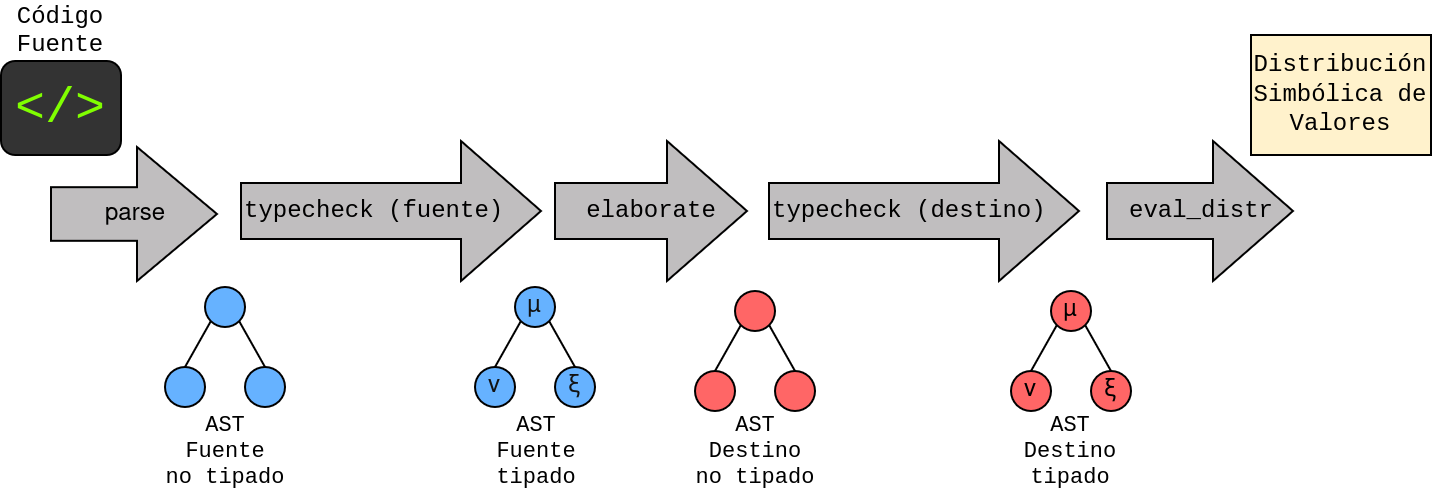
\includegraphics[width=\linewidth]{img/pipeline.png}
  \caption{Pipeline principal del intérprete.}
  \label{fig:pipeline}
\end{figure}



\section{Módulos y sus interacciones}

La figura \ref{fig:modulos} muestra la organización de los módulos y submódulos del intérprete. A continuación, se describe la responsabilidad principal de cada módulo.


\begin{figure}
  \centering
  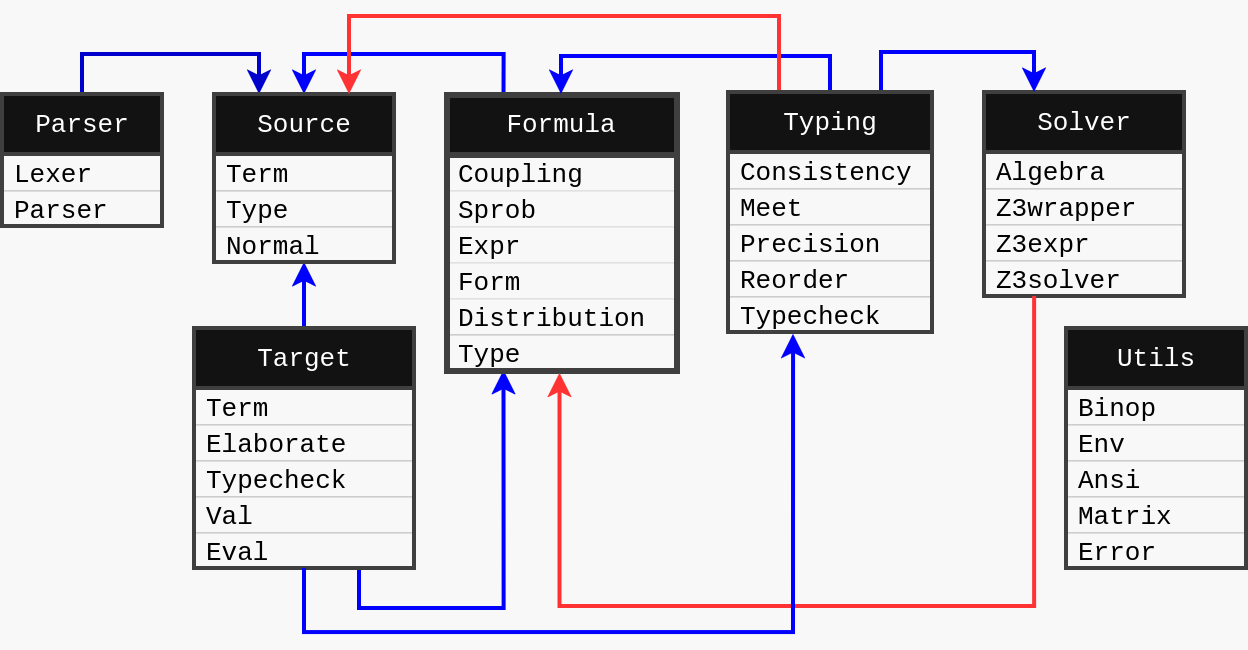
\includegraphics[width=0.8\linewidth]{img/dependency.png}
  \caption{Módulos y submódulos del intérprete.}
  \label{fig:modulos}
\end{figure}


\subsection{Parser} El módulo \verb|Parser| está encargado del procesamiento del archivo
con código fuente de GPLC. Sus dos submódulos \verb|Parser.Lexer| y
\verb|Parser.Parser| toman la responsabilidad de realizar los
análisis léxico y sintático de un programa, recibido por la entrada
estándar. El primer submódulo tiene como dependencia externa la
librería \verb|OCamllex|, un generador de analizadores
léxicos, y el segundo depende de la librería \verb|Menhir|, otra
librería robusta usada para la generación de analizadores sintáticos.
Como dependencia interna, el módulo \verb|Parser| depende del módulo
\verb|Source|, del cual obtiene las estructuras de datos y rutinas para
llevar a cabo la construcción del AST fuente no tipado.

\subsection{Source} El módulo \verb|Source| contiene todas las
estructuras de datos que constituyen el lenguaje fuente. Mientras que
\verb|Source.Type| define los tipos graduales simples y de
distribución y las probabilidades graduales, \verb|Source.Term| define la sintaxis abstracta de las expresiones del lenguaje fuente.

\subsection{Formula} El módulo \verb|Formula| es el responsable de
definir toda la infraestructura simbólica de la aplicación. En él,
el módulo \verb|Formula.Distribution| define qué es una distribución
simbólica, y tiene como dependencia \verb|Formula.Form| que define
las fórmulas que controlan las probabilidades de una distribución
simbólica. Este último submódulo depende a su vez de \verb|Formula.Expr|, que define el álgebra de las expresiones
que participan en las fórmulas. Finalmente, \verb|Formula.Expr| depende de \verb|Formula.Sprob| que es el módulo que define la probabilidad simbólica, la cual junto con los números participa en las expresiones que conforman las restricciones en las fórmulas. El submódulo \verb|Formula.Type| define los tipos de fórmula simples y de distribución, estos últimos usando la distribución simbólica paramétrica definida en \verb|Formula.Distribution| para implementar la distribución de tipos de fórmula simples. Adicionalmente, es el módulo \verb|Type| el que implementa la rutina para \emph{levantar} los tipos graduales a tipos de distribución.

\subsection{Solver} El módulo \verb|Solver| está a cargo de los
juicios de satisfacibilidad de las fórmulas definidas por el módulo
\verb|Formula|. El submódulo \verb|Solver.Algebra| define inductivamente
sus propias expresiones, similares a aquellas definidas por \verb|Formula.Expr|, e implementa transformaciones para convertir las fórmulas de \verb|Formula| a ecuaciones/inecuaciones nativas del módulo \verb|Solver.Algebra|. De este modo, un cambio de implementación solo implica una modificación de los transformadores, y no una modificación general del mecanismo de resolución. El submódulo \verb|Solver.Z3expr| utiliza los transformadores definidos en \verb|Solver.Z3wrapper| para traducir las ecuaciones e inecuaciones de \verb|Solver.Algebra| a expresiones nativas de la librería \verb|Z3|.
Para terminar, el submódulo \verb|Solver.Z3solver| contiene la función \verb|solve|, encargada de determinar la satisfacibilidad de una fórmula del módulo \verb|Formula|, la cual puede recibir directamente como argumento y transformar a expresión de Z3 gracias a las funcionalidades de transformación del módulo \verb|Solver|. De esta manera, \verb|solve| se constituye como el punto de integración del intérprete con Z3.


\subsection{Typing} El módulo \verb|Typing| es el encargado de la
definición de todas las operaciones entre tipos que se realizan en el
procesamiento del intérprete, y además implementa la rutina de chequeo
estático de tipos del lenguaje fuente. El submódulo \verb|Consistency|
implementa el juicio de consistencia para los tipos graduales en
\verb|Source.Type| y de fórmula en \verb|Formula.Type|. Los submódulos
\verb|Meet| y \verb|Precision| definen la operación de cómputo del
ínfimo y el juicio de precisión entre tipos de fórmula. Las
operaciones de consistencia, precisión e ínfimo hacen uso de las
estructuras que provee el módulo \verb|Formula.Coupling|, que modela
en función de las fórmulas de las distribuciones argumento, el sistema
de restricciones discutido en la sección \ref{par:symbolic},
retornando un sistema de restricciones cuya satisfacibilidad determina si
la operación del ínfimo está o no definida, o si los juicios de
consistencia y precisión son verdaderos o falsos. Las restricciones
provistas por \verb|Formula.Coupling| son resueltas en \verb|Z3|
mediante el pipeline descrito en el párrafo del módulo
\verb|Solver|. Finalmente, el submódulo \verb|Typecheck| es el que
realiza el proceso estático de tipado del AST fuente recibido del
módulo de \emph{parsing}.

\subsection{Target} En el módulo \verb|Target| se definen todas las
estructuras de datos y rutinas esenciales del lenguaje destino. El submódulo \verb|Term| define el AST del lenguaje destino. A diferencia
del módulo \verb|Source| que tiene un submódulo \verb|Type| donde define sus propios tipos (graduales), el módulo \verb|Target| deriva los suyos de \verb|Formula.Type|. \verb|Elaborate| es el submódulo a cargo de la elaboración (descrita en la sección \ref{sec:elab}), es decir, de la transformación del AST fuente tipado producido por \verb|Typing.Typecheck| a un AST destino no tipado cuya forma está definida por \verb|Term|. \verb|Typecheck| implementa el chequeo estático de tipos sobre el AST producido por la elaboración. El submódulo \verb|Val| define los valores crudos, valores y distribuciones de valores del lenguaje destino (descritos en la sección \ref{sec:target-language}). Finalmente, \verb|Eval| define la rutina que efectúa la evaluación del AST tipado, retornando una distribución simbólica de valores, con la forma definida en \verb|Val|.


\subsection{Resumen de dependencias}
Las dependencias entre módulos se muestran en la
figura~\ref{fig:modulos} mediante flechas, cuya punta indica el módulo
del cual se depende. Se omiten las dependencias asociadas a
\verb|Utils|, pues este módulo provee funcionalidades transversales a
todo el sistema.

En conjunto, estas dependencias reflejan la forma en que se organiza
el procesamiento de un programa dentro del intérprete. \verb|Parser|
depende de \verb|Source| para construir el AST fuente. \verb|Formula|
depende de \verb|Source| para hacer el \emph{levantamiento} de tipos
graduales a tipos de fórmula. \verb|Typing| depende de \verb|Source|
para tipar el AST fuente y operar sobre tipos graduales, de
\verb|Formula| para manipular tipos de fórmula, y de \verb|Solver|
para verificar la satisfacibilidad de las fórmulas involucradas. Por
su parte, \verb|Solver| depende de \verb|Formula| para traducir
fórmulas a expresiones nativas de Z3, mientras que \verb|Target|
depende de \verb|Source| para elaborar, a partir del AST fuente, el
AST destino, y de \verb|Typing| para ejecutar operaciones sobre tipos
de fórmula.




\section{Estructuras de datos}
En esta sección se presentan las estructuras de datos fundamentales del
intérprete. En particular, se describen los AST de los lenguajes fuente
y destino, los tipos graduales y los tipos de fórmula, y los entornos que permiten
asociar identificadores con tipos o valores en el proceso de tipado
y la evaluación.

\subsection{AST fuente}
El AST fuente es una estructura de datos implementada en el módulo
\verb|Source.Term|, y que modela la primera representación intermedia
del programa. Esta estructura tiene la flexibilidad adecuada al lugar
central que ocupa en la arquitectura de la aplicación, dado que
gracias a un parámetro de tipo, puede representar los AST no tipados
que produce la fase de \emph{parsing}, y luego representar los nodos
tipados con una anotación simple o de distribución, que devuelve el
chequeo estático efectuado por el módulo \verb|Typing.Typecheck|. El
AST fuente contiene además un objeto de metadatos, con la información
posicional de las expresiones del AST en el código fuente, lo cual es
fundamental para el reporte más útil de errores, mensajes de advertencia,
o un trabajo de depuración más informado.

\subsection{AST destino}
El AST destino está implementado en el módulo \verb|Target.Term|. Es
la estructura que constituye la segunda representación intermedia del
programa.  Tiene en común con su contraparte fuente el hecho de ser
una estructura paramétrica que se adapta tanto al requerimiento de
construir un AST no tipado (por ejemplo el que produce la fase
elaboración), como al de construir un AST con anotaciones de tipo (por
ejemplo, el que produce el chequeo estático del módulo
\verb|Target.Typecheck|). Al igual que el AST fuente, el AST destino
tiene un componente con metadatos, que en cada nodo preserva la
información posicional de cada nodo en el código fuente.


\subsection{Tipos graduales} Los tipos graduales
\verb|Source.Type.simple| y \verb|Source.Type.distr| modelan los tipos
usados en la sintaxis concreta del lenguaje. Por lo tanto, sus
constructores son usados en la fase de parsing para construir las
anotaciones (ascripciones) de tipo realizadas en el código fuente.
Forman parte integral de los nodos fuente, no solo en las sintaxis
abstracta de las ascripciones, sino también en la anotación de tipo en
cada nodo, hecha durante el chequeo estático. Las probabilidades
graduales no especificadas, también definidas en el módulo
\verb|Source.Type|, portan un identificador numérico
relevante para la arquitectura, pues una probabilidad desconocida se
propaga por la estructura del intérprete como una probabilidad
simbólica, y el identificador ayuda a asignar en distintas
instancias una misma variable para una probabilidad \verb|?|.

\subsection{Tipos de fórmula} Los tipos de fórmula
\verb|Formula.Type.simple| y \verb|Formula.Type.distr| modelan los
tipos usados exclusivamente en el lenguaje destino y en las
operaciones de tipo presentes en el módulo \verb|Typing|. El uso que
las operaciones de tipos hacen de estos está fundamentado en el poder
simbólico que le permite a las operaciones plantear el sistema de
restricciones descrito en la sección \ref{par:symbolic}. En el AST
destino, tanto las ascripciones (tipo ascrito y evidencia) como las
anotaciones por nodo realizadas en el chequeo estático utilizan tipos
de fórmula. Por último, estos tipos también son usados en el chequeo
dinámico de tipos de valores, efectuado en el módulo
\verb|Target.Eval|.

\subsection{Entornos} La última estructura de datos fundamental del
intérprete es el entorno, un mapa que permite
recuperar un objeto en función de un identificador. Las dos utilidades
que el entorno presta son {(1)} recuperar el tipo simple de una
variable durante los chequeos estáticos fuente
(\verb|Typing.Typecheck|) y destino (\verb|Target.Typecheck|), y
{(2)} recuperar el valor de una variable durante el proceso de
evaluación del AST tipado (\verb|Target.Eval|).

\section{Rutinas principales}

Las estructuras de datos descritas en la sección anterior son las
entradas y salidas de un conjunto de rutinas que, en el nivel más alto
del intérprete, representan las fases principales de procesamiento del
código fuente.

\subsection{Parsing} Esta rutina es la responsable de la
transformación del código fuente de un programa sintácticamente válido
de GPLC a un AST fuente no tipado, y de registrar en cada nodo que
construye la información posicional de inicio y término de la
expresión procesada.

\begin{center}
  \texttt{Código Fuente}
  $\rightarrow$
  \fbox{\texttt{parse}}
  $\rightarrow$
  \texttt{AST no tipado}
\end{center}


\subsection{Tipado fuente} Esta rutina del módulo \verb|Typing.Typecheck| recibe un AST fuente no tipado,
y retorna una estructura de la misma clase, pero con cada nodo portando un tipo simple o de distribución, inferido e insertado ahí por el chequeo estático de tipos. En esta rutina, se hace un uso recurrente  de \verb|Typing.Consistency| para verificar los juicios de consistencia propios del tipado gradual.
\begin{center}
  \texttt{AST Fuente no tipado}
  $\rightarrow$
  \fbox{\texttt{Typing.Typecheck.typecheck}}
  $\rightarrow$ \texttt{AST Fuente tipado}
\end{center}

\subsection{Elaboración} Esta transformación toma un AST fuente tipado, es decir, que cumple con el invariante de contener anotaciones de tipo en todos sus nodos, y transforma la expresión fuente en cada nodo a su expresión correspondiente en el lenguaje destino, retornando un AST destino no tipado. Sin embargo, la transformación también introduce explícitamente en el AST que construye, nuevas ascripciones con evidencia (además de las que introduce como traducción de las ascripciones del lenguaje fuente), por lo que el AST destino, en general, no tiene la misma estructura que el fuente. La elaboración depende
en gran parte de la operación \verb|Typing.Meet.meet| (ínfimo) para determinar las evidencias de casi todas las ascripciones que introduce en la nueva estructura. Esta fase preserva los metadatos de posición de cada nodo, propagando la información posicional hacia la ascripción que introduce para ese nodo.
\begin{center}
  \texttt{AST Fuente tipado}
  $\rightarrow$
  \fbox{\texttt{Target.Elaborate.elaborate}}
  $\rightarrow$
  \texttt{AST Destino no tipado}
\end{center}





\subsection{Tipado destino} Esta rutina verifica que después de la
elaboración el AST esté bien construido y siga cumpliendo con las reglas
estáticas de consistencia. Tras verificar las reglas de consistencia
establecidas para cada tipo de expresión, utilizando la consistencia
basada en evidencia (\verb|Precision.transitive_consistency_simple| y
\verb|Precision.transitive_consistency|), la rutina infiere un tipo
para cada nodo y lo anota en el espacio reservado en la estructura del
AST, retornando un AST destino tipado.  En el diseño de este
intérprete, la decisión de inferir el tipo de cada nodo destino y
anotarlo en el AST se fundamenta en el hecho de que una regla
central de la semántica operacional que reduce los programas a valores
--la reducción de la ascripción de distribución
$\eascr{\epsilon}{m}{\nu}$-- demanda conocer el tipo $\mu$ de la
subexpresión ascrita $m$, para definir la asignación de evidencias y
ascripciones simples a los valores de la distribución $\Vdistr$ a la
cual se evalúa $m$.
\begin{center}
  \texttt{AST Destino no tipado}
  $\rightarrow$
  \fbox{\texttt{Target.Typecheck.typecheck}}
  $\rightarrow$
  \texttt{AST Destino tipado}
\end{center}



\subsection{Evaluación}
Finalmente, en la fase de evaluación, la rutina
\verb|Target.Eval.eval_distr_value| toma el AST destino tipado, y
reduce cada uno de sus nodos a una distribución de valores. Las
distribuciones de valores de las subexpresiones se combinan de
distintas formas para llegar a producir una distribución simbólica de
valores, cuya fórmula es el resultado de la acumulación de las
fórmulas surgidas durante el proceso de evaluación. Si el programa
termina, la fórmula que restringe las variables de la distribución se
garantiza satisfacible.
\begin{center}
  \texttt{AST Destino Tipado}
  $\rightarrow$
  \fbox{\texttt{Target.Eval.eval\_distr\_value}}
  $\rightarrow$
  \texttt{Dis. simbólica de val.}
\end{center}


     % 6 sec/arquitectura.tex
% -*- TeX-master: "../main.tex" -*-


\chapter{Implementación}
\label{sec:implementacion}
El enfoque de este capítulo es presentar la implementación de las principales estructuras que dan soporte a las operaciones del intérprete, y las rutinas esenciales que operan sobre ellas. Entre las estructuras de datos, se cubren los tokenes de código fuente, ambos AST (fuente y destino), los tipos graduales, los tipos de fórmula y la infraestructura simbólica como parte integral de ellos, y los valores que el sistema retorna. Las principales rutinas que se tratan son parsing de código fuente, operaciones de tipo, resolución de fórmulas, chequeo estático de ambos AST, elaboración,  y evaluación.

\section{Estructuras de datos}


En esta sección se presentan las principales estructuras de datos del
intérprete a través de sus implementaciones en OCaml. Los
fragmentos de código que se muestran corresponden a definiciones
reales de tipos dentro de los módulos del sistema. Usualmente se
denota con \verb|t| el tipo principal definido por un módulo. La
palabra clave \verb|and| se utiliza para realizar definiciones
mutuamente inductivas. El uso de \verb|of| en un constructor indica el
tipo de los valores que recibe, y \verb|*| se utiliza para formar
productos (tuplas) de tipos. Finalmente, \lstinline{|} separa los
distintos constructores de un tipo. A continuación, se introducen las
implementaciones de los tipos graduales, ambos AST, los tipos de
fórmula, la infraestructura simbólica asociada y los valores del
lenguaje.

\subsection{Tipos graduales}

La probabilidad gradual en el lenguaje fuente es un componente de la expresión de selección y de los tipos de distribución. No es un tipo en sí mismo, pero por ser parte integral de los tipos graduales, se implementa en el módulo \verb|Source.Type| como el tipo de dato  algebraico \verb|gprob|, que contempla constructores para la probabilidad concreta y la desconocida. En la sintaxis de OCaml, el constructor de la probabilidad concreta \verb|Preal| toma un número de punto flotante (la probabilidad) y un entero (un id). El constructor de la probabilidad desconocida \verb|Pany| toma solo un entero, que también representa un id, y es de particular importancia para convertir una probabilidad \verb|?| a una única probabilidad simbólica en distintas instancias de transformación.

Los tipos graduales simples y de distribución están implementados como dos tipos de datos algebraicos mutuamente inductivos: el constructor funcional del tipo simple, \verb|Fun|, toma como argumento el par \verb|(simple, distr)|, y el constructor básico de distr, \verb|Distr|, toma como argumento una lista de pares \verb|(simple, gprob)|.  El resto de los constructores del tipo simple son
\verb|Real|, \verb|Bool| y \verb|Any|, este último representando al tipo desconocido \verb|?|. Los demás constructores del tipo de distribución son \verb|Scale| y
\verb|Sum|, los cuales escalan una distribución por una probabilidad gradual, y suman una lista de distribuciones, respectivamente.

\begin{ocamlblock}[caption={Probabilidad Gradual y Tipos Graduales},label={asdf}]
type gprob  = (* probabilidad gradual *)
| Preal of float * int (* Uso: Preal(probabilidad: float, id: int)*)
| Pany of int 

type simple = (* tipos graduales simples *)
| Real | Bool
| Any  | Fun of simple * distr

and distr = (* tipos graduales de distribución *)
| Distr of (simple * gprob) list (* Uso: Distr [(t1,p1); ... ; (tn,pn)] *) 
| Scale of gprob * distr 
| Sum   of distr list
\end{ocamlblock}


\subsection{AST fuente}

El AST del lenguaje fuente está implementado en el
módulo \verb|Source.Term| como un tipo de datos algebraico inductivo. Este es un
tipo parametrizado por dos variables de tipo \verb|'st| y \verb|'dt|. Sus
constructores modelan la sintaxis abstracta del lenguaje fuente. Cada
constructor a su vez recibe como último argumento un valor de otro tipo
paramétrico: la anotación \verb|'t annot|, en la cual se inserta el tipo del
nodo, una vez inferido por el chequeo estático.

El fundamento de parametrizar el tipo \verb|ast| con dos variables de tipo es lograr utilizar
esta misma estructura para modelar los AST no tipados y tipados: Si se parametriza
ast con el par de tipos (\verb|(unit,unit)|), entonces la anotación hereda el tipo \verb|unit|
y el espacio reservado para el tipo del nodo se llena con el único valor de este tipo, es decir, \verb|()|.
En cambio si el tipo \verb|ast| se parametriza con el par \verb|(simple,distr)|, cada anotación recibirá
uno de estos dos tipos. Cuál de los dos tipos asignar a una anotación determinada es una decisión
que está codificada en la definición del \verb|ast|. Por ejemplo, la anotación de la expresión \verb|Num|
es del tipo \verb|'st annot|, lo cual significa que recibirá un tipo simple. En cambio,
la anotación de la expresión \verb|Choice| tiene tipo \verb|'dt annot|, indicando que recibirá un
 tipo de distribución. Este diseño apunta a resolver la tensión entre un AST no tipado y uno tipado,
y entre la asignación de distintas categorías de tipo a nodos de un mismo AST.

\begin{ocamlblock}[caption={AST lenguaje fuente},label={lst:lst:src-ast}]
type ('st, 'dt) ast =
| Num       of float * 'st annot
| Bool      of bool * 'st annot 
| Var       of string * 'st annot
| Fun       of string * Type.simple * ('st,'dt) ast * 'st annot
| Sascr     of ('st,'dt) ast * Type.simple * 'st annot
| Dascr     of ('st,'dt) ast * Type.distr * 'dt annot
| Let       of string * ('st,'dt) ast * ('st,'dt) ast list * 'dt annot 
| If        of ('st,'dt) ast * ('st,'dt) ast * ('st,'dt) ast * 'dt annot
| App       of ('st,'dt) ast * ('st,'dt) ast * 'dt annot 
| Choice    of Type.gprob * ('st,'dt) ast * ('st,'dt) ast * 'dt annot 
| NumBinOp  of ('st,'dt) ast * ('st,'dt) ast *  Bin.num_op * 'st annot 
| BoolBinOp of ('st,'dt) ast * ('st,'dt) ast * Bin.bool_op * 'st annot 

type untyped_term = (unit,unit) ast
type typed_term   = (simple,distr) ast\end{ocamlblock}

\subsection{Fórmulas}
Las fórmulas son sistemas de ecuaciones e inecuaciones, posiblemente no
lineales, cuyas variables corresponden a probabilidades simbólicas de
distribuciones de fórmula.

En la base del concepto de fórmula, está la
probabilidad simbólica, implementada como un constructor \verb|SymProb| que toma
4 argumentos: un primer argumento string, que es la variable de la probabilidad
simbólica propiamente tal, un segundo argumento de tipo entero, que indica la
posición de la probabilidad dentro de la distribución, y finalmente dos
argumentos más de tipo entero, que almacenan, según sea el origen de la
distribución, información acerca de la posición dentro de la distribución o
información de las posiciones de los tipos simples que dieron origen a la
probabilidad en la distribución producto.

El tipo de dato algebraico que modela las expresiones que se comparan en las
fórmulas se implementa en \verb|Formula.Expr|. Los constructores \verb|Real| y
\verb|Symb| elaboran los casos base de esta álgebra. El primero toma un número real, y el segundo una probabilidad
simbólica. En particular, el
constructor \verb|Symb| transforma una probabilidad simbólica en una expresión
simbólica. \verb|Add|, \verb|Sub|, \verb|Mul| y \verb|Div| son las operaciones
reales binarias básicas. \verb|Sum| y \verb|Prod| suman y multiplican listas de
expresiones, respectivamente.

El tipo de datos \verb|Formula.Form.t| es el que representa a las fórmulas como
restricciones, y como conjunciones entre estas mismas.  Los constructores
\verb|Integrity|, \verb|Distribution| y \verb|Null| aplican a una expresión,
restricciones importantes, y por eso reciben nombres significativos. Los
constructores \verb|Eq|, \verb|Lt| y \verb|Le| comparan dos expresiones con
las relaciones $=$, $<$ y $\leq$. Finalmente, el operador de conjunción
\verb|And| le da su carácter inductivo al tipo de fórmula, representando una
conjunción sobre una lista de fórmulas.



\begin{ocamlblock}[caption={Fórmulas y sus componentes},label={lst:formula}]
  (* probabilidad simbólica (módulo: Sprob) *)
  type t = SymProb of string * int * int * int (* Uso: TagVar("X",5,1,4) *)

  (* expresión simbólica (módulo: Expr) *)
  type t =
  | Real  of float  | Symb  of Sprob.t
  | Add   of t * t  | Sub   of t * t
  | Mul   of t * t  | Div   of t * t
  | Sum   of t list | Prod  of t list

  (* fórmula (módulo: Form) *)
  type t = 
  | Integrity    of Expr.t (* expresión en [0,1] *)
  | Distribution of Expr.t (* expresión = 1.0 *)
  | Null         of Expr.t (* expresión = 0.0*)
  | Eq           of Expr.t * Expr.t (* expr1 = expr2 *)
  | Lt           of Expr.t * Expr.t (* expr1 < expr2 *)
  | Le           of Expr.t * Expr.t (* expr1 <= expr2 *)
  | And          of t list (* And[f1;...;fn] *)
\end{ocamlblock}





\subsection{Distribución paramétrica y tipos de fórmula}
En el módulo \verb|Formula.Distribution| se implementa el tipo
paramétrico de distribución \verb|dis|. Este tipo materializa la idea
de la distribución de fórmula como un tipo polimórfico consistente en
un par \emph{(distribución, fórmula)}, donde la distribución es una
lista de pares de tipo \verb|(t', Sprob.t)|, es decir, valores de tipo
\verb|t'| asociados a una probabilidad simbólica. La fórmula asociada
a la distribución impone restricciones a los valores posibles de las
probabilidades de tipo \verb|Sprob.t|. El tipo \verb|'t| representa el
\emph{dominio} de la distribución.

La implementación de los tipos de fórmula es similar a la de los tipos
graduales. Los tipos simples y de distribución son también definidos de manera
mutuamente inductiva. Los tipos simples, producidos por los constructores
\verb|Real|, \verb|Bool|, \verb|Any| y \verb|Fun(simple,distr)| son análogos a
aquellos en los tipos graduales. La diferencia fundamental radica en los tipos de
distribución: estos se definen como el tipo \verb|dis|, parametrizado por el
tipo \verb|simple|. De esta manera, el tipo \verb|distr| es efectivamente
definido como una distribución simbólica de tipos simples. 

\begin{ocamlblock}[caption={Distribución Paramétrica y Tipos de Fórmula}, label={lst:ftype}]
  (* tipo polimórfico de distribución (módulo: Distribution) *)
  type 't dis = (('t * Sprob.t) list) * Form.t

  (* tipos de fórmula simples *)
  type simple = 
  | Real
  | Bool
  | Any 
  | Fun of simple * distr

  (* tipos de fórmula de distribución *)
  and distr = simple Distribution.dis
\end{ocamlblock}


\subsection{AST destino}
El AST destino, implementado en \verb|Target.Term|, es muy semejante al AST del
lenguaje fuente, dado que también se define de manera paramétrica para
adaptarse a los requerimientos previos y posteriores al chequeo estático del
lenguaje destino. El componente de tipo \verb|'t annot| es el mismo tipo usado
en los nodos del AST fuente, dado que el parámetro \verb|'t| puede ser
cualquier tipo (simple o distribución, gradual o de fórmula). Esto facilita
además la propagación de información posicional desde el lenguaje fuente al
destino, ya que los metadatos dentro de la anotación son trasladados por defecto
a su nodo destino durante la elaboración.

En el Código~\ref{lst:trgt-ast} se muestra un extracto de la
definición de los nodos del AST destino, incluyendo solo aquellos
que se diferencian de sus nodos correspondientes en el lenguaje
fuente.  Los constructores \verb|Sascr| y \verb|Dascr|, que producen
las expresiones de ascripción simple y de distribución,
respectivamente, ahora reciben un primer argumento adicional, que
constituye la evidencia de la ascripción. El constructor de
\verb|Choice|, a diferencia de su versión fuente, recibe dos
probabilidades simbólicas: la de selección de la primera rama, y su
complemento. El tipo \verb|fprob| es en realidad un tipo definido
como \verb|type fprob = Sprob.t * Form.t|, es decir, una probabilidad
simbólica $x$ asociada a una fórmula $x=r$ o $0\leq x \leq 1$.


Análogo a lo hecho en el lenguaje fuente, los tipos de expresión no tipada y
tipada se definen parametrizando el AST polimórfico con los pares de tipos
\verb|(unit,unit)| y \verb|(simple,distr)|, respectivamente.

\begin{ocamlblock}[caption={AST destino (extracto)}, label={lst:trgt-ast}]
  type ('s,'d) t =
  ...
| Sascr        of fsimple * ('s,'d) t * fsimple * 's annot
| Dascr        of fdistr  * ('s,'d) t * fdistr  * 'd annot
| Choice       of ('s,'d) t * ('s,'d) t * fprob * fprob * Form.t * 'd annot
| Let          of string  * ('s,'d) t * ('s,'d) t list * 's list * 'd annot

type untyped_term = (unit,unit) t
type typed_term   = (fsimple,fdistr) t
\end{ocamlblock}

\subsection{Valores}

En el módulo \verb|Target.Val| se definen los tipos de datos para los
valores retornados por el intérprete. El tipo de valor más básico es
el valor crudo, que puede ser un número, un booleano o una clausura
(el valor de una expresión lambda). Este último valor conserva en su
estructura el ambiente de definición, por lo que las funciones en esta
implementación tienen \emph{alcance léxico}, es decir, una variable toma
su valor del entorno donde fue definida.

El tipo \verb|value| corresponde al valor que figura asociado a una
probabilidad en las distribuciones de valor retornadas por el
intérprete. El constructor de valor \verb|Ascr| representa una
ascripción de tipo simple (tercer argumento) sobre el valor crudo
(segundo argumento) contenido en el valor. El primer argumento es otro tipo
simple que funciona como evidencia de la ascripción.

La distribución de valores es definida mediante el mismo tipo
paramétrico \verb|dis| utilizado para definir los
tipos de fórmula de distribución. En este caso el tipo \verb|dis|
recibe como parámetro el tipo \verb|value|, lo que resulta en una
distribución simbólica sobre valores del lenguaje, con una fórmula que
restringe sus variables.

\begin{ocamlblock}[caption={Valor Crudo, Valor, y Distribución de Valores}, label={lst:val}]
  (* valor crudo *)
  type raw_value = 
  | Num of float * val_id 
  | Bool of bool * val_id
  | Closure of (string * simple * typed_term * env) * val_id

  (* valor *)
  and value = 
  | Ascr of simple * raw_value * simple 
  | Error of simple
  
  (* distribución de valores *)
  type distr_value = value Formula.Distribution.dis
\end{ocamlblock}

\section{Rutinas} En esta sección se presentan las principales rutinas
ejecutadas por la implementación en el procesamiento de un programa de
GPLC. En particular, se describen las rutinas de lexing y parsing, el
chequeo estático del AST fuente, las operaciones de tipo, la
resolución de fórmulas simbólicas mediante el solucionador, y la elaboración
del programa fuente a su representación correspondiente en el lenguaje
destino. Aunque el pipeline completo del intérprete también contempla
un chequeo estático del AST destino, su presentación se omite pues su
implementación es muy similar a la del chequeo fuente. Por su mayor
complejidad, la implementación de la evaluación se omite en esta
sección.

\subsection{Lexing y parsing}

El análisis léxico del intérprete fue implementado haciendo uso de la
librería generadora de analizadores léxicos Ocamllex. Los
archivos implementados como artefactos para que dicha librería genere
el módulo \verb|Lexer| son:
\begin{itemize}
\item Un archivo con la implementación de un tipo de dato algebraico
  denominado \verb|token|, cuyos constructores son una representación
  abstracta de las unidades léxicas que se espera encontrar en el
  texto. La mayoría de los constructores no contiene más que dos
  argumentos de información posicional: el inicio y el final del
  lexema en el texto. En cambio constructores como \verb|NUM| (número) o
  \verb|IDENT| (identificador) portan la información específica que le da
  a un token su expresividad. El primer constructor porta un número de punto
  flotante, y el segundo un string (el identificador o variable)
\item Un archivo con la definición de una regla que retorna un token,
  mediante \emph{pattern matching} sobre expresiones regulares, que se
  comparan con los lexemas encontrados en el texto. En casos como el de
  reconocimiento de un número en el texto, el número se pasa como un argumento
  al constructor del token \verb|NUM|, además de la información posicional.
  El caso del token \verb|LAMBDA| muestra que más de un lexema puede ser asociado
  un token.
\end{itemize}

\begin{ocamlblock}[caption={Implementación de \texttt{token} y reconocimiento de lexemas},label={lst:imp-parse}]
  type token =
  ...
  | NUM        of (float  * Lexing.position * Lexing.position)
  | IDENT      of (string * Lexing.position * Lexing.position)
  | LAMBDA     of (Lexing.position * Lexing.position)
  | TRUE       of (Lexing.position * Lexing.position)

  rule token = parse
  ...
  | decimal {
    let sp = Lexing.lexeme_start_p lexbuf in
    let ep = Lexing.lexeme_end_p   lexbuf in
    NUM (Float.of_string decimal, sp, ep)
  }
  ...
  | "lambda" | "lambda!" { 
    let sp = Lexing.lexeme_start_p lexbuf in
    let ep = Lexing.lexeme_end_p   lexbuf in
    LAMBDA(sp, ep)
  }
\end{ocamlblock}

El parser se implementó con la librería Menhir, a partir de un archivo
\verb|parser.mly| donde se declara la gramática del lenguaje. Esta
gramática describe cómo una secuencia de tokens (producidos por el
lexer) se transforma en expresiones del lenguaje: cada token incluye sus
posiciones (de tipo \verb|Lexing.position|), de modo que el parser puede
construir recursivamente el AST fuente con los constructores provistos
por \verb|Source.Term| y, al mismo tiempo, registrar en cada nodo su
rango posicional dentro del código fuente.  Durante el parsing, algunas
reglas de producción, como la de probabilidad gradual y la de tipos de
distribución, se someten a chequeos semánticos para verificar su
validez.


\subsection{Operaciones de tipo}

Las operaciones de tipo más relevantes que se implementan en este
intérprete son las que determinan la consistencia, precisión, y el
ínfimo entre dos tipos. Las siguientes razones justifican limitar la
exposición a las operaciones entre tipos de fórmula:
\begin{itemize}
\item La única operación que se usa en tipos graduales es la consistencia
\item Los tipos graduales de distribución se deben convertir antes a tipos de fórmula
  para determinar su consistencia, por lo que la operación de consistencia para tipos
  graduales de distribución no es más que convertirlos a tipos de fórmula y luego aplicar
  la versión de fórmula de la operación entre los tipos convertidos
\item La consistencia entre tipos graduales simples se implementa de manera análoga
  entre tipos simples de fórmula.
\end{itemize}

Para tipos simples o de distribución, las operaciones de consistencia
y precisión toman dos tipos de la misma categoría
(\verb|(simple,simple)| o \verb|(distr,distr)|) y retornan un valor de
tipo \verb|bool|, que indica el valor lógico de la proposición. En el
caso del meet, se retorna un tipo \verb|'t option|, donde \verb|'t| es
el tipo de los argumentos: Por ejemplo, si los argumentos son de tipo
\verb|simple|, entonces el resultado puede ser \verb|Some Real|, en el
caso de que el resultado exista y sea \verb|Real|, y \verb|None| en
caso contrario.  Las versiones de estas operaciones para tipos
simples son una traducción directa de la formulación original del
lenguaje, codificando, mediante \emph{pattern matching}, los resultados
para cada par de tipos.

La consistencia simple recibe dos tipos simples \verb|t1| y
\verb|t2|. El \emph{pattern matching} sobre el par \verb|(t1,t2)| retorna
\verb|true| para los pares \verb|(Any,_)| y \verb|(_,Any)|, donde
\verb|_| es cualquier tipo. También se retorna \verb|true| para los
casos \verb|(Real,Real)| y \verb|(Bool,Bool)|. El caso del par
\verb|(Fun(s1,d1),Fun(s2,d2))| retorna el valor \verb|b1 && b2|,
donde \verb|b1| es la consistencia simple entre \verb|s1| y \verb|s2|,
y \verb|b2| es la consistencia de distribución entre \verb|d1| y
\verb|d2|.

La operación de precisión retorna \verb|true| para los pares
\verb|(Real,Real)| y \verb|(Bool,Bool)|. El par \verb|(_,Any)| retorna
\verb|true| (todo tipo es tanto o más preciso que $\Any$). Siguiendo el
patrón de la consistencia, la precisión retorna
\verb|(Fun(s1,d1),Fun(s2,d2))| si la precisión simple entre s1 y s2, y
la precisión de distribución entre d1 y d2 retornan \verb|true|.


La operación de meet simple retorna un tipo opcional: si entre los tipos argumento está definida la relación de precisión, se retorna el constructor \verb|Some| con el tipo más preciso. Si los dos tipos no son comparables, la operación no está definida y se retorna \verb|None|. Concretamente si uno de los dos tipos es el desconocido \verb|Any|, se retorna por defecto \verb|Some| con el otro tipo. Para los tipos \verb|(Real,Real)| y \verb|(Bool,Bool)| se retorna \verb|Real| y \verb|Bool|, respectivamente.
Siguiendo el patrón recursivo de las operaciones anteriores,
para el par de tipos \verb|(Fun(s1,d1),Fun(s2,d2))| se retorna \verb|Some Fun(s3,d3)|, donde \verb|s3| es el tipo obtenido del meet simple entre \verb|s1| y \verb|s2|, y \verb|d3| es el tipo en el meet de distribución entre \verb|d1| y \verb|d2|. Si cualquiera de los dos meet recursivos retorna \verb|None|, entonces el meet entre funciones también lo hace.

Para los tipos de distribución de fórmula, las tres operaciones (\verb|consistency|, \verb|precision| y \verb|meet|) siguen un mismo patrón, basado en construir un acoplamiento simbólico entre las probabilidades de ambas distribuciones. Si $d_1=(\{(s_i,p_i)\}_i,\Phi_1)$ y $d_2=(\{(t_j,q_j)\}_j,\Phi_2)$, se crea una matriz de variables frescas $\alpha_{ij}$ (módulo \verb|Formula.Coupling|) y se impone: (i) \emph{compatibilidad por celda} ($\alpha_{ij}$ debe ser nula cuando $s_i$ no es compatible con $t_j$), (ii) \emph{marginales} ($p_i=\sum_j \alpha_{ij}$ y $q_j=\sum_i \alpha_{ij}$), y (iii) las fórmulas originales $\Phi_1$ y $\Phi_2$. El solucionador decide la satisfacibilidad del sistema; en consistencia/precisión eso determina el valor booleano, y en meet, si es satisfacible, el soporte del resultado se obtiene filtrando las celdas definidas (las que retornan \verb|Some|) y asociándoles su peso $\alpha_{ij}$.

Para los tipos de distribución de fórmula, las tres operaciones siguen
un mismo patrón de diseño e implementación (ilustrado en el Algoritmo~\ref{alg:typeop}), basado en la construcción
de un coupling $\coupling$, es decir, una matriz de variables. La
primera tarea es determinar qué variables $\alpha_{ij}$ deben ser
iguales a 0 por la incompatibilidad de los tipos simples $\sigma_i$ y
$\delta_j$ de las distribuciones en cuestion. Para discernir esto se
define, a modo de \emph{máscara}, la matrix $R$ con entrada $i,j$ el
resultado \verb|meet_simple|$(\sigma_i,\delta_j)$ en el caso de la
operación meet, y el valor lógico \verb|rel|$(\sigma_i,\delta_j)$
cuando \verb|rel| es la consistencia o la precisión. De esta manera,
las funciones \verb|Coupling.alpha_option_formula| y
\verb|Coupling.alpha_bool_formula|, toman como argumento el par
$(R,\coupling)$ y retornan la fórmula que contiene la condición
correcta para cada $\alpha_{ij}$: Si
\verb|meet_simple|$(\sigma_i,\delta_j)$ está definido, o
\verb|rel|$(\sigma_i,\delta_j)$ es verdadero, entonces
$0<=\alpha_{ij}<= 1$ (es una variable libre) dentro de la fórmula. De
lo contrario, $\alpha_{ij} = 0$. La segunda tarea es imponer a cada
fila de la matriz $\coupling$ sumar lo mismo que su probabilidad
simbólica correspondiente, es decir, $p_i = \sum_j\alpha_{ij}$. También
se debe imponer una condición análoga para las columnas y las
probabilidades $q_j$. Las fórmulas que codifican estas restricciones
para filas y columnas de $\coupling$ son retornadas
\verb|Coupling.row_sum_formula| y \verb|Coupling.col_sum_formula|
respectivamente, que toman como argumento el arreglo de probabilidades
correspondiente y $\coupling$. La fórmula $\Phi$ que agrupa en
conjunción la fórmula de restricciones individuales sobre variables
$\alpha_{ij}$, las fórmulas de suma de filas y columnas, y las dos
fórmulas $\Phi_1$ y $\Phi_2$, heredadas de las distribuciones $\mu$ y
$\nu$, es la fórmula cuya satisfacibilidad indica si el meet está definido,
o si las relaciones son verdaderas. La función
\verb|Solver.Z3solver.solve| es aplicada sobre la fórmula $\Phi$, y si
la fórmula tiene solución, entonces en este punto la consistencia y
precisión retornan \verb|true|. De lo contrario retornan
\verb|false|. Si $\Phi$ tiene solución y se trata de meet, entonces la
función \verb|Coupling.filter_alpha_option| retorna una distribución
con las entradas no nulas en la matriz $R$ asociadas a sus pesos
correspondientes en la matriz $\coupling$. Esta distribución y la
fórmula $\Phi$ son envueltos en \verb|Some| y retornados. En cambio si
la fórmula $\Phi$ no tiene solución, se retorna \verb|None|


\begin{algorithm}[H]
\caption{Patrón común para operaciones sobre tipos de distribución}
\label{alg:typeop}
\KwIn{
  $\mu=([(\sigma_i,p_i)]_i,\Phi_1)$, $\nu=([(\delta_j,q_j)]_j,\Phi_2)$,
  $\mathtt{op}\in\{\mathtt{Cons},\mathtt{Prec},\mathtt{Meet}\}$
}
\KwOut{\texttt{bool} (Cons/Prec) o \texttt{Option}$(D,\Phi)$ (Meet)}

$\coupling \leftarrow \texttt{Coupling.create}(m,n)$ \tcp*{Coupling con variables frescas $\alpha_{ij}$}

\tcp{R es matriz máscara de op sobre los tipos $\sigma_i$ y $\delta_j$}
$R \leftarrow [\,\texttt{op}(\sigma_i,\delta_j)\,]_{ij}$ \tcp*{R puede contener tipo simple option o bool según op}

\BlankLine


$\Phi \leftarrow \Phi_1 \land \Phi_2$ \tcp*{$\Phi$ es la fórmula a resolver}
\lIf{$\mathtt{op}=\mathtt{Meet}$}
{$\Phi \leftarrow \Phi \land \texttt{Coupling.alpha\_option\_formula}(\coupling,R)$}

\lElse{$\Phi \leftarrow \Phi \land \texttt{Coupling.alpha\_bool\_formula}(\coupling,R)$}
$\Phi \leftarrow \Phi \land \texttt{Coupling.row\_sum\_formula}([p_i]_i,\coupling)$\;
$\Phi \leftarrow \Phi \land \texttt{Coupling.col\_sum\_formula}([q_j]_j,\coupling)$\;
\BlankLine

\If{\texttt{solve}$(\Phi)$}{
  \uIf{$\mathtt{op}\neq\mathtt{Meet}$}{
    \Return \texttt{true}\;
  }
  \Else{
    $D \leftarrow \texttt{Coupling.filter\_alpha\_option}(R,\coupling)$;
    
    $\xi \leftarrow (D,\Phi)$;
    
    \Return \texttt{Some} $\xi$\;
  }
}
\Else{
  \uIf{$\mathtt{op}\neq\mathtt{Meet}$}{
    \Return \texttt{false}\;
  }
  \Else{
    \Return \texttt{None}\;
  }
}
\end{algorithm}


\subsection{Resolución de fórmulas}
\label{sec:impl-rutinas-solver}

La función \verb|Solver.Z3solver.solve| (Algoritmo~\ref{alg:solve}) es
el punto de conexión del intérprete con el solucionador Z3. Esta
función recibe una lista de fórmulas (de tipo \verb|Formula.Form.t|) y
retorna un valor lógico: \verb|true| si el sistema tiene una solución
en los números reales, y \verb|false| si no existe una
solución. En algunos casos, por ejemplo si la fórmula
  excede la capacidad computacional del solucionador o si una fórmula
  está mal estructurada, el proceso de resolución puede no terminar.
  Para evitar ejecuciones sin término, la lista de configuración
  \verb|cfg=[("model","false"); ("timeout","20000")]| impone un tiempo
  máximo de 20 segundos (20000 milisegundos), tras el cual Z3
  interrumpe la búsqueda por \emph{timeout}. Además, la opción
  \verb|("model","false")| desactiva la generación de modelos (la
  construcción de una solución particular), ya que en este intérprete
  no se instancia la solución en probabilidades reales concretas.


En la implementación de \verb|solve|, la lista de
fórmulas recibida como argumento se transforma a una lista de
expresiones nativas de la librería \verb|Z3|. Esta transformación se
realiza mediante la función auxiliar \verb|formula_to_z3expr|
(Algoritmo~\ref{alg:formula-to-z3expr}), que traduce cada fórmula del
intérprete a una expresión de Z3.

Un aspecto importante de esta traducción es el \emph{contexto} de Z3.
La función \verb|formula_to_z3expr| toma como argumento una fórmula y un
contexto \verb|ctx|. Este contexto agrupa la información necesaria para
construir y tipar expresiones dentro de una invocación al solucionador,
por lo tanto todas las transformaciones de fórmulas dentro de
\verb|solve| deben usar un mismo contexto.

En particular, \verb|formula_to_z3expr| primero utiliza
\verb|Algebra.of_formula| para obtener una restricción expresada en un tipo de datos interno del módulo \verb|Solver| a partir
de la fórmula, y luego utiliza \verb|Z3expr.of_constr| para convertir
dicha restricción en una expresión nativa de \verb|Z3|. El resultado
corresponde a igualdades/desigualdades cuyas variables son heredadas de
las probabilidades simbólicas presentes en la fórmula original.



\begin{algorithm}[H]
\caption{\texttt{Solver.Z3solver.formula\_to\_z3expr}}
\label{alg:formula-to-z3expr}
\KwIn{$\Phi$ : \texttt{Formula.Form.t}, $ctx$ : \texttt{Z3.context}}
\KwOut{$e$ : \texttt{Z3expr.t}}

$c \leftarrow \texttt{Algebra.of\_formula}(\Phi)$;

$e \leftarrow \texttt{Z3expr.of\_constr}(c,ctx)$ \tcp*{genera una expresión nativa de Z3}
\Return $e$\;
\end{algorithm}


Una vez obtenida la lista de expresiones de Z3, \verb|solve| intenta
resolver el sistema con dos solucionadores. El primero es un
solucionador de Z3 configurado para la lógica
\texttt{QF\_LRA}\footnote{QF significa \emph{quantifier-free}
  (sin cuantificadores). LRA es \emph{linear real
    arithmetic}: aritmética real lineal, es decir, restricciones sobre
  reales sin productos entre
  variables como $x\cdot y$.}. Si el chequeo retorna \verb|SAT|
(\emph{satisfiable}), entonces \verb|solve| retorna \verb|true|,
indicando que el sistema tiene solución. Por otro lado, si el chequeo
retorna \verb|UNSAT| (\emph{unsatisfiable}), entonces \verb|solve|
retorna \verb|false|.

Si el chequeo resulta en \verb|UNKNOWN|, entonces se prueba con un
segundo solucionador de Z3 configurado para la lógica
\texttt{QF\_NRA}\footnote{NRA es \emph{nonlinear real
    arithmetic}: aritmética real no-lineal, es decir, permite productos entre variables como $x\cdot y$
  o potencias como $x^2$).}.  En este caso, \verb|solve| retorna
\verb|true| si el chequeo encuentra una solución, y retorna
\verb|false| en cualquier otro caso, para señalar que no existe una
solución en los reales para el sistema.


El resultado de \verb|solve| es recibido en un contexto donde se decide
qué hacer con su valor retornado pero, típicamente, \verb|true|
significa que una relación entre distribuciones se verifica o que una
operación entre distribuciones está bien definida. Por otro lado,
\verb|false| suele significar que se levantará una excepción.

\begin{algorithm}[H]
\caption{\texttt{solve}}
\label{alg:solve}
\KwIn{$[\Phi_i]_i$ : lista de \texttt{Formula.Form.t}}
\KwOut{\texttt{bool}}

$\mathit{cfg} \leftarrow \{(\texttt{\strquote{model}},\texttt{\strquote{false}}),(\texttt{\strquote{timeout}},\texttt{\strquote{20000}})\}$\tcp*{configuración}
$ctx \leftarrow \texttt{Z3.mk\_context}(\mathit{cfg})$\tcp*{contexto}

$E \leftarrow [\,\texttt{formula\_to\_z3expr}(\Phi_i,ctx)\,]_i$\tcp*{Lista de expresiones}

$s_1 \leftarrow \texttt{mk\_solver}(ctx,\texttt{\strquote{QF\_LRA}})$\tcp*{Solucionador lineal}
\texttt{add}$(s_1, E)$;

$r_1 \leftarrow \texttt{check}(s_1)$\;

\If{$r_1 = \texttt{SAT}$}{\tcp*{$\Phi$ tiene solución}
  \Return \texttt{true}\;
}
\ElseIf{$r_1 = \texttt{UNSAT}$}{\tcp*{$\Phi$ NO tiene solución}
  \Return \texttt{false}\;
}
\Else{ \tcp*{$r_1 = \texttt{UNKNOWN}$}
  $s_2 \leftarrow \texttt{mk\_solver}(ctx,\texttt{\strquote{QF\_NRA}})$\tcp*{Solucionador NO lineal}
  \texttt{add}$(s_2, E)$\;
  $r_2 \leftarrow \texttt{check}(s_2)$\;

  \If{$r_2 = \texttt{SAT}$}{
    \Return \texttt{true}\;
  }
  \Else{
    \Return \texttt{false}\;
  }
}
\end{algorithm}

\subsection{Tipado fuente}
\label{sec:impl-rutinas-tc-fuente}

La rutina de chequeo estático del lenguaje fuente (Algoritmo~\ref{alg:tc-fuente}) está implementada en
el módulo \verb|Typing.Typecheck| mediante la función recursiva
\verb|Typing.Typecheck.typecheck|. Esta función recibe un AST fuente
no tipado y un entorno, inicialmente vacío, que asocia identificadores a tipos
simples graduales, y retorna un AST de la misma estructura, pero con
una anotación de tipo insertada en cada nodo. En esta fase, por lo
tanto, el programa no es transformado a otra representación, sino
reconstruido preservando sus metadatos y reemplazando la anotación
vacía de cada constructor por el tipo gradual inferido para la
expresión correspondiente.

La rutina sigue de cerca las reglas estáticas presentadas en la
sección~\ref{sec:abstract-gplc}. Su funcionamiento general consiste en
descender recursivamente por el AST, chequear primero las
subexpresiones, recuperar a partir de ellas los tipos ya inferidos
mediante \verb|get_simple_type| y \verb|get_distr_type|, y usar
dichos tipos para decidir si el nodo actual es estáticamente válido.
Las decisiones de aceptación o rechazo se apoyan principalmente en las
operaciones de consistencia del módulo \verb|Typing.Consistency|, en las
operaciones auxiliares sobre tipos graduales de \verb|Source.Type|, y
en el manejo del entorno provisto por \verb|Utils.Env|.

Un caso particularmente importante es el de \verb|Let|. Como en GPLC
la expresión ligada puede representar una distribución de tipos, la
implementación primero normaliza el tipo de distribución inferido para
la expresión nombrada, obtiene de esa forma la lista de pares
\verb|(tipo, probabilidad)|, y luego chequea el cuerpo una vez por
cada tipo simple posible de la variable ligada. Cada una de estas
instancias produce un tipo de distribución para el cuerpo, y el tipo
del bloque completo se reconstruye como la suma de dichas
distribuciones, escaladas por las probabilidades originales de la
expresión ligada. De este modo, la implementación materializa
directamente la semántica iterativa que el \verb|let| tiene en la
formulación del lenguaje.


\begin{algorithm}
\caption{Tipado Estático Fuente: \texttt{Typing.Typecheck.typecheck} (Extracto)}
\label{alg:tc-fuente}
\KwIn{$t$ (AST fuente no tipado), $\Gamma$ (entorno de tipos simples)}
\KwOut{$t'$ (AST fuente tipado)}
$md \leftarrow \mathtt{meta}(t)$\tcp*{metadatos con información posicional de nodo no tipado}
\tcp{Pattern matching sobre expresiones de AST}
\If{$t = \mathtt{Num}(n,\_)$}{
  \Return $\mathtt{Num}(n,\mathtt{Annot}(Real,md))$\;
}

\ElseIf{$t = \mathtt{Var}(x,\_)$}{
  $\sigma \leftarrow \mathtt{lookup}(\Gamma,x)$\;
  \Return $\mathtt{Var}(x,\mathtt{Annot}(\sigma,md))$\;
}



\ElseIf{$t = \mathtt{Dascr}(m,\nu,\_)$}{
  $m' \leftarrow \mathtt{typecheck}(m,\Gamma)$\;
  $\mu \leftarrow \mathtt{distrType}(m')$\;
 
  \If{$\mathtt{gradual\_distr\_consistency}(\nu,\mu)$ \tcp{Chequeo de consistencia}}{ 
    \Return $\mathtt{Dascr}(m',\nu,\mathtt{Annot}(\nu,md))$\;
  }
  \Else{
    \textbf{raise} \texttt{Exception};
  }
}

\ElseIf{$t = \mathtt{Choice}(p,m,n,\_)$}{
  $m' \leftarrow \mathtt{typecheck}(m,\Gamma)$;  $n' \leftarrow \mathtt{typecheck}(n,\Gamma)$\;
  $\mu \leftarrow \mathtt{distrType}(m')$;  $\nu \leftarrow \mathtt{distrType}(n')$\;
  $q \leftarrow \mathtt{prob\_compl}(p)$ \tcp*{complemento}
  $\tau \leftarrow \mathtt{Sum}([\mathtt{Scale}(p,\mu),\mathtt{Scale}(q,\nu)])$\;
  \Return $\mathtt{Choice}(p,m',n',\mathtt{Annot}(\tau,md))$\;
}

\ElseIf{$t = \mathtt{Let}(x,m,[n],\_)$}{
  $m' \leftarrow \mathtt{typecheck}(m,\Gamma)$\;
  $\mu \leftarrow \mathtt{distrType}(m')$\;
 
  $[(\sigma_i,p_i)]_i \leftarrow \mathtt{normalize\_distr}(\mu)$ \tcp*{-> lista de (tipo,prob)}
  $\Gamma_i \leftarrow \mathtt{extend}(\Gamma,x,\sigma_i)$ \tcp*{un entorno por cada tipo posible de $x$}
  $n'_i \leftarrow \mathtt{typecheck}(n,\Gamma_i)$\;
  $\nu_i \leftarrow \mathtt{distrType}(n'_i)$\;
  $\tau \leftarrow \mathtt{Sum}([\mathtt{Scale}(p_i,\nu_i)]_i)$\;
  \Return $\mathtt{Let}(x,m',[n'_i]_i,\mathtt{Annot}(\tau,md))$\;
}




\tcp*{otros casos}

\Else{

   \textbf{Error} \;
}
\end{algorithm}


\subsection{Elaboración}
\label{sec:impl-rutinas-elaboracion}

La elaboración corresponde a la traducción desde el AST fuente
tipado (producido por \verb|typecheck| del módulo \verb|Target.Typecheck|) hacia
un AST destino no tipado, implementada en el módulo
\verb|Target.Elaborate| mediante la rutina recursiva
\verb|Target.Elaborate.elaborate|. El objetivo de esta fase no es
volver a inferir tipos, sino \emph{reformular} el programa en un
lenguaje destino que haga explícitas las verificaciones dinámicas y la
infraestructura simbólica (probabilidades simbólicas y fórmulas)
requeridas en tiempo de ejecución.

En términos de implementación, la elaboración efectúa los
siguientes cambios: {(1)} Cada nodo destino (incluyendo nodos
nuevos introducidos por la transformación) hereda los metadatos del
nodo fuente correspondiente, de modo que los errores reportados en
fases posteriores puedan localizarse con precisión.  {(2)} Los
tipos graduales anotados en el AST fuente se transforman a tipos de
fórmula del lenguaje destino (mediante las fórmulas
\lstinline|lift_simple| y \lstinline|lift_distr|), lo cual hace
explícito el componente simbólico.  {(3)} Cada ascripción del
lenguaje destino (\lstinline|Sascr| / \lstinline|Dascr|) porta una
evidencia, computada como el ínfimo entre el tipo inferido de la
subexpresión y el tipo esperado.

Un aspecto importante es que, dado que el AST fuente ya fue chequeado
estáticamente, la elaboración asume que los \emph{meet} necesarios
están definidos. En consecuencia, un fallo al calcular evidencia se
interpreta como un error interno de la implementación (o una violación
de invariantes), y no como un error atribuible al programa del
usuario.

El Algoritmo~\ref{alg:elab} muestra un extracto de casos
representativos.  Los casos omitidos (por ejemplo, operadores,
\lstinline|let|, ascripción de distribución, etc.)  siguen el mismo
patrón: recursión, levantamiento de tipos, cómputo de evidencia
mediante {meet}, y reconstrucción del nodo destino preservando
metadatos.


\begin{algorithm}[H]
\caption{Elaboración: \texttt{Target.Elaborate.elaborate} (extracto)}
\label{alg:elab}
\KwIn{$t$ (AST fuente tipado)}
\KwOut{$u$ (AST destino no tipado)}
$md \leftarrow \mathtt{meta}(t)$; \tcp*{metadatos del nodo fuente}
$ann \leftarrow \mathtt{Annot}((),md)$; \tcp*{anotación destino (sin tipo, solo metadatos)}

\If{$t = \mathtt{Num}(n,\_)$}{
  \Return $\mathtt{Sascr}(Real,\ \mathtt{Num}(n,ann),\ Real,\ ann)$\;
}

\ElseIf{$t = \mathtt{Var}(x,\_)$}{
  \Return $\mathtt{Var}(x,ann)$\;
}



\ElseIf{$t = \mathtt{Dascr}(m,\nu,\_)$}{
  $\mu \leftarrow \texttt{distrType}(m)$\tcp*{tipo gradual de expresión fuente}
  $\mu' \leftarrow \mathtt{lift\_distr}(\mu)$; $\ \nu' \leftarrow \mathtt{lift\_distr}(\nu)$\tcp*{tipos grad -> tipos de fórm.}
  $m' \leftarrow \mathtt{elaborate}(m)$\tcp*{elaboración de m}
  $\epsilon \leftarrow \mathtt{meet\_distr}(\mu',\nu')$\tcp*{se asume definido}
  \Return $\mathtt{Dascr}(\epsilon,\ m',\ \nu',\ ann)$\;
}

\ElseIf{$t = \mathtt{Choice}(p,m,n,\_)$}{
  $\mu \leftarrow \mathtt{distrType}(m)$; $\ \nu \leftarrow distrType\mathtt{}(n)$;
  
  $m' \leftarrow \mathtt{elaborate}(m)$; $\ n' \leftarrow \mathtt{elaborate}(n)$;
  
  $\mu' \leftarrow \mathtt{lift\_distr}(\mu)$; $\ \nu' \leftarrow \mathtt{lift\_distr}(\nu)$\;

  $(\alpha,\Phi_\alpha) \leftarrow \mathtt{lift\_gprob}(p)$\tcp*{prob. simbólica + restricciones}
  $(\omega,\Phi_{\omega}) \leftarrow \mathtt{complement}(\alpha)$\;
  $\Phi \leftarrow \Phi_\alpha \land \Phi_{\omega} \land (\alpha + \omega = 1)$;

  $\tau_1 \leftarrow \mathtt{add\_formula}(\alpha \cdot \mu' + \omega\cdot\nu', \Phi )$\;

  $\tau_2 \leftarrow \mathtt{lift\_distr}(\mathtt{distrType}(t))$\tcp*{tipo gradual inferido del nodo}
  $\epsilon \leftarrow \mathtt{meet\_distr}(\tau_1,\tau_2)$\tcp*{se asume definido}

  $c \leftarrow \mathtt{Choice}(m',n',(\alpha,\Phi_\alpha),(\omega,\Phi_\omega),\Phi,ann)$\;
  \Return $\mathtt{Dascr}(\epsilon,\ c,\ \tau_2,\ ann)$\;
}

\tcp*{otros casos}

\Else{

   \textbf{Error} \;
}
\end{algorithm}
   % 7 sec/implementacion.tex
% -*- TeX-master: "../main.tex" -*-

\chapter{Validación}\label{sec:validacion}



El fin de este capítulo es presentar un conjunto de casos que cumplen
un doble propósito: {(1)} aportar evidencia de que el intérprete
implementa correctamente el lenguaje GPLC y {(2)}  ilustrar el
uso práctico del lenguaje mediante programas pequeños pero
representativos.  La evidencia obtenida se basa en el contraste entre
los resultados producidos por el intérprete y el comportamiento
esperado: en los casos exitosos, las distribuciones retornadas y sus
valores con ascripción, y en los casos fallidos, los diagnósticos de
error reportados. Como complemento, al final del capítulo se incluye
una subsección de limitaciones que sintetiza dificultades observadas
durante la implementación y que motivan trabajo futuro.

A diferencia de una verificación formal completa, la validación que se
presenta aquí es funcional y dirigida por casos.  Cada programa está
diseñado para cubrir una expresión específica (o una interacción
acotada entre expresiones) y contrastar el comportamiento observado
con las reglas y decisiones de diseño descritas en capítulos previos.
Este enfoque resulta adecuado para GPLC, ya que lo que se busca
contrastar se refleja en hechos directamente observables: la
aceptación de programas bien formados y la producción de
distribuciones con valores y tipos coherentes; la propagación de
probabilidades concretas y desconocidas de acuerdo con las reglas del
lenguaje; y el rechazo estático o dinámico de programas inválidos
mediante diagnósticos precisos con localización y explicación de la
inconsistencia detectada.

Finalmente, estos casos también cumplen un rol ilustrativo, ya que
muestran patrones de uso propuestos, ejemplos mínimos y casos de borde
que aclaran qué se acepta, qué se rechaza y por qué. Por ello, el
capítulo está organizado en torno a familias de expresiones, agrupando
los programas por la construcción que se desea validar.


\section{Metodología}

Para cada caso se documentan tres elementos: {(1)} el código
fuente GPLC, {(2)} la salida del intérprete (ya sea una
distribución simbólica o un mensaje de error), y {(3)} una
explicación breve del aspecto que se está validando. En los casos
exitosos, la validación se apoya en observar que: {(i)} el
programa es aceptado por el chequeo estático, {(ii)} la
distribución retornada contiene los valores esperados, y
{(iii)} los tipos que figuran en cada valor son los
correctos. En los casos fallidos, se espera un rechazo estático o
dinámico según corresponda, y se valida que el intérprete reporte el
error con un mensaje informativo y una localización adecuada.

Los ejemplos se seleccionan además para cubrir el \emph{carácter
  gradual} del lenguaje: probabilidades desconocidas \verb|?|, el tipo
desconocido \verb|?|, y el efecto de estos elementos en consistencia,
ascripción y construcción de distribuciones. Con esto, el capítulo
busca evidenciar no solo que el intérprete evalúa programas, sino
también que preserva las restricciones semánticas y de integridad que
motivan el diseño de GPLC para escenarios con incertidumbre e
información parcial.



\section{Casos}

Los casos se organizan por construcción sintáctica: selección
probabilística para distribuir probabilidad entre dos ramas,
\lstinline|let| para definir variables, lambdas para abstracción y
aplicación, \lstinline|if| para control y ascripción para imponer
tipos. Cada conjunto de casos reúne programas mínimos que aíslan el
comportamiento bajo estudio, y luego incorpora ejemplos donde la
interacción entre componentes graduales (tipos y probabilidades
desconocidas) es relevante. Cuando corresponde, también se incluyen
casos de rechazo estático y dinámico para ilustrar las condiciones
bajo las cuales el intérprete protege la integridad semántica de
probabilidades y distribuciones.

\subsection{Selección binaria probabilística} El Código
\ref{lst:choice1} muestra un caso elemental de selección
probabilística: la selección de un número real con probabilidad
concreta 0.5. La salida muestra una distribución simbólica donde los
elementos 1 y 0 están ascritos por el tipo \lstinline|Real|, y
ponderados por probabilidades simbólicas.


\begin{gplcblock}[caption={Selección de números reales},label={lst:choice1}]
0.5 $ 1 : 0

>>>

{
	 [Real] 1. :: Real : SymProb19 ,
	 [Real] 0. :: Real : SymProb20 
}   
\end{gplcblock}




El Código \ref{lst:choice2} muestra un caso de selección con ramas
no homogéneas: valores de tipo \lstinline|Real| y \lstinline|Bool| son
seleccionados, lo cual constituye una decisión de diseño importante:
Las ramas no necesitan ser de un mismo tipo. Además la selección es
hecha con una probabilidad incógnita. La variable simbólica libre
asociada a dicha probabilidad queda internamente codificada en la
fórmula de la distribución retornada.

  
\begin{gplcblock}[caption={Selección de booleano y número},label={lst:choice2}]
? $ true : 10

>>>

{
	 [Bool] true :: Bool : SymProb19 ,
	 [Real] 10. :: Real : SymProb20 
}  
\end{gplcblock}

El Código \ref{lst:choice3} muestra un ejemplo de selección anidada,
es decir, una selección con una rama que, a su vez,
es una selección. En la salida se observa cómo los
tres valores conforman el soporte de la distribución
retornada.

\begin{gplcblock}[caption={Selección anidada},label={lst:choice3}]
0.4 $ (? $ true : false) : 10

>>>

{
	 [Bool] true :: Bool : SymProb71 ,
	 [Bool] false :: Bool : SymProb72 ,
	 [Real] 10. :: Real : SymProb73 
}  
\end{gplcblock}



En el Código \ref{lst:choice4}, la expresión de selección tiene una
ascripción de tipo de distribución que verifica estáticamente su
consistencia con el tipo inferido de la expresión. En la distribución
ascrita, el tipo \lstinline|Real| concentra el peso total de los
elementos reales, lo cual comprueba que en la relación de consistencia
la distribución de los pesos de un tipo no afecta la consistencia
entre las distribuciones. Por lo tanto, el resultado de un juicio de
consistencia está determinado estrictamente por relaciones semánticas
entre los tipos, sin importar la sintaxis específica. Esto es cierto
en general para todas las relaciones y operaciones entre
distribuciones.

\begin{gplcblock}[caption={Selección con ascripción},label={lst:choice4}]
(0.5 $ 1 : (0.4 $ 0 : false)) :: {Real : 0.7 , Bool : 0.3}

>>>

{
	 [Real] 1. :: Real : SymProb46 ,
	 [Real] 0. :: Real : SymProb47 ,
	 [Bool] false :: Bool : SymProb48 
}  
\end{gplcblock}
  
Con un carácter más gradual, los Códigos \ref{lst:choice5.1},
\ref{lst:choice5.2} y \ref{lst:choice5.3} muestran la flexibilidad que
se logra con el tipo desconocido \lstinline|?| y la probabilidad
desconocida \lstinline|?|.  El Código \ref{lst:choice5.1} muestra
que el tipo \lstinline|?| --consistente con los tipos \lstinline|Real|
y \lstinline|Bool|-- puede distribuir su peso entre \lstinline|Real| y
\lstinline|Bool| para lograr la consistencia con el tipo de la
expresión. El Código \ref{lst:choice5.2} evidencia que la
distribución con probabilidades desconocidas es consistente con toda
expresión cuyo tipo sea una distribución de \lstinline|Real| y
\lstinline|Bool|, o incluso una distribución con solo uno de esos dos
tipos, ya que la probabilidad \lstinline|?| es compatible con 0.0, es
decir, puede representar también la probabilidad de un tipo con peso
nulo. Finalmente, el Código \ref{lst:choice5.3} demuestra que se
puede anotar la selección con cualquier distribución de
\lstinline|Real| y \lstinline|Bool|, dado que la selección con
probabilidad desconocida es consistente con distribución de pesos en
tipo de ascripción.


\begin{gplcblock}[caption={Distribución con tipo no especificado},label={lst:choice5.1}]
(0.3 $ true : (-1)) :: {Bool : 0.2, ? : 0.8}

>>>

{
	 [Bool] true :: Bool : SymProb21 ,
	 [Bool] true :: ? : SymProb22 ,
	 [Real] -1. :: ? : SymProb23 
}  
\end{gplcblock}

\begin{gplcblock}[caption={Distribución con probabilidades no especificadas},label={lst:choice5.2}]
(0.3 $ true : (-1)) :: {Real : ?, Bool : ?}

>>>

{
	 [Bool] true :: Bool : SymProb21 ,
	 [Real] -1. :: Real : SymProb22 
}  
\end{gplcblock}

\begin{gplcblock}[caption={Ascripción de selección con prob. \texttt{?}},label={lst:choice5.3}]
(? $ true : (-1)) :: {Real : 0.5 , Bool : 0.5}

>>>

{
	 [Bool] true :: Bool : SymProb21 ,
	 [Real] -1. :: Real : SymProb22 
}  
\end{gplcblock}



Para demostrar con claridad el funcionamiento efectivo del mecanismo
estático de tipado, se analizan un par de casos donde la ascripción
impuesta a la selección gatilla un error estático.

En el Código \ref{lst:choice6}, la ponderación exacta que tiene el
tipo \lstinline|Bool| en la distribución inducida por la selección, es
exactamente \lstinline|0.4|. Sin embargo, en la ascripción, el tipo
`Bool` tiene una ponderación más alta.


\begin{gplcblock}[caption={Inconsistencia por prob. de \texttt{Bool}},label={lst:choice6}]
(0.4 $ false : lambda x:?.x) :: {Bool:0.45 , ?:?}

>>>

Static Error [line 1, cols 1-49]: In distribution ascription, type 0.4 * ({Bool:1}) + 0.6 * ({? -> {?:1}:1}) of term inconsistent with ascription type {Bool:0.45, ?:?}
\end{gplcblock}

Para terminar, el Código \ref{lst:choice7} falla porque en la
anotación no hay ningún tipo consistente con el tipo funcional
\lstinline|Real -> {Real:1}| que represente su peso \lstinline|0.5| en
el tipo de distribución ascrito.




\begin{gplcblock}[caption={Inconsistencia por falta de tipo funcional},label={lst:choice7}]
(0.5 $ lambda x:Real.1 : false) :: {Bool : ? , Real : ?}

>>>

Static Error [line 1, cols 1-56]: In distribution ascription, type 0.5 * ({Real -> {Real:1}:1}) + 0.5 * ({Bool:1}) of term inconsistent with ascription type {Bool:?, Real:?}
\end{gplcblock}

\subsection{Let}
La semántica de la operación \lstinline|let| consiste en asignar a la
variable \lstinline|x| cada uno de los elementos contenidos en la
distribución implícita de la expresión nombrada, y luego establecer
una distribución de probabilidad que contenga las instancias del
cuerpo con cada versión de variable \lstinline|x|. La probabilidad de
cada valor asignado a \lstinline|x|, dentro de la distribución ligada,
se toma como el peso del cuerpo en la distribución resultante.

En el primer ejemplo (Código \ref{lst:let1}), el programa es semánticamente
equivalente a la expresión \lstinline|(0.3 $ true : 1)|. La
distribución de valores retornada muestra la combinación
probabilística efectiva del cuerpo del \verb|let| (simplemente la variable
\verb|x|), evaluado en todo el rango de la variable. La variable funciona como en la mayoría de los lenguajes cuando la
expresión nombrada representa solo un elemento. Por ejemplo, en los casos
\lstinline|y = false| o \lstinline|id = lambdax:?.x|.

\begin{gplcblock}[caption={Definición de variable local},label={lst:let1}]
let x = (0.3 $ true : 1) in x

>>>

{
	 [Bool] true :: Bool : SymProb41 ,
	 [Real] 1. :: Real : SymProb42 
}  
\end{gplcblock}

El mayor potencial del bloque \lstinline|let| consiste naturalmente en
la operabilidad que le otorga a los elementos de una variable de
distribución.  En el Código \ref{lst:let2.1}, la variable b es el
argumento de una operación lógica, y en el Código \ref{lst:let2.2}
la variable r participa en una operación aritmética. Aunque no sea
visible en los pesos simbólicos, la variable propaga a la distribución
resultante el peso probabilístico de los valores individuales
asignados a ella.


\begin{gplcblock}[caption={Uso de variable en operación lógica},label={lst:let2.1}]
let b = (0.9 $ true : false) in (true or b)

>>>

{
	 [Bool] true :: Bool : SymProb73 ,
	 [Bool] true :: Bool : SymProb74 
}  
\end{gplcblock}



\begin{gplcblock}[caption={Uso de variable en operación aritmética},label={lst:let2.2}]
let r = (? $ 0 : 10) in (7 * r)

>>>

{
	 [Real] 0. :: Real : SymProb73 ,
	 [Real] 70. :: Real : SymProb74 
}  
\end{gplcblock}

El Código \ref{lst:let3} muestra bloques \lstinline|let| anidados.
Dada la naturaleza semántica de la expresión \lstinline|let|, la
expresión final en términos de \lstinline|n| y \lstinline|b| combina
todos los valores posibles de las variables, cuatro combinaciones en
total. Además, el programa se verifica con la ascripción de un tipo de
distribución consistente con la equiprobabilidad de \lstinline|Real| y
\lstinline|Bool|.




\begin{gplcblock}[caption={Bloques \texttt{let} anidados},label={lst:let3}]
(let n = (? $ 1 : 7) in
let b = (0.3 $ true : false) in
(0.5 $ 21 / n : b and false))  :: {Real:0.5, Bool:0.5}

>>>

{
	 [Real] 21. :: Real : SymProb403 ,
	 [Bool] false :: Bool : SymProb404 ,
	 [Real] 21. :: Real : SymProb405 ,
	 [Bool] false :: Bool : SymProb406 ,
	 [Real] 3. :: Real : SymProb407 ,
	 [Bool] false :: Bool : SymProb408 ,
	 [Real] 3. :: Real : SymProb409 ,
	 [Bool] false :: Bool : SymProb410 
}  
\end{gplcblock}

El ejemplo del Código~\ref{lst:let4} exhibe elementos importantes de la expresión
\lstinline|let| en conexión con las expresiones \lstinline|lambda|. Es
conveniente la asignación de una lambda a una variable, pues
permite una aplicación mucho menos verbosa y más práctica que la
aplicación de una lambda literal directamente al argumento. En segundo
lugar, el programa demuestra la capacidad del bloque \lstinline|let|
para extraer funciones de una selección.  La ascripción verifica que
los resultados son exclusivamente de tipo \lstinline|Real|.


\begin{gplcblock}[caption={Asignación de lambda a variable},label={lst:let4}]
(let step_forward = lambdax.x+1 in
let step_back = lambday.y-1 in
let f = (? $ step_forward : step_back) in
(f 0)) :: {Real:1.0}

>>>

{
	 [Real] 1. :: Real : SymProb145 ,
	 [Real] -1. :: Real : SymProb146 
}  
\end{gplcblock}

En el contexto de los bloques \lstinline|let| y las expresiones
lambda, es pertinente mencionar que si se usa una variable que no ha
sido definida con los medios que la sintaxis ofrece, como la
asignación de una expresión en un bloque \lstinline|let|, o como
parámetro formal de una expresión lambda, entonces el intérprete
gatilla un error cuyo mensaje especifica cuál es la variable no
definida, y la ubicación exacta del código en que fue utilizada.  En
el Código \ref{lst:invalid-var} se muestra el uso inválido de la
variable \lstinline|x| en el cuerpo de la expresión lambda.

\begin{gplcblock}[caption={Uso de variable no definida},label={lst:invalid-var}]
lambda y : Bool . (x + y)

>>>

Static Error [line 1, cols 19-20]: variable x not found
\end{gplcblock}


\subsection{Lambda}

\begin{comment}
Las expresiones lambda tienen la sintaxis
\lstinline|lambda<var>:<simple>.<expr>|.  La
sintaxis\lstinline| lambda<var>.<expr>| es azúcar sintático de
\lstinline|lambda<var>:?.<expr>|. Si bien el argumento de una función
debe ser una expresión de tipo simple, es decir, un valor (número,
booleano, variable, o lambda), el cuerpo de la función puede ser
cualquier clase de expresión.
\end{comment}

Las expresiones lambda tienen la sintaxis
\lstinline|lambda <var> : <simple> . <expr>|. La
sintaxis \lstinline|lambda <var> . <expr>| es
azúcar sintáctico para
\lstinline|lambda <var> : ? . <expr>|.  Si bien el argumento de una función
debe ser una expresión de tipo simple, es decir, un valor (número,
booleano, variable, o lambda), el cuerpo de la función puede ser
cualquier clase de expresión.

En el programa del Código~\ref{lst:lambda1.1}, la función
\lstinline|seven_untyped| tiene un parámetro formal de tipo
\lstinline|?|.  Por lo tanto, la función es capaz de recibir un
argumento con cualquier tipo simple, sin levantar un error estático de
inconsistencia, porque \lstinline|?| es consistente con todo tipo
simple. (En el caso particular de esta función, tampoco sería posible
tener un error dinámico, porque el cuerpo no tiene la variable como
subexpresión). Los argumentos 1 y true se pasan exitosamente y el
programa termina.

\begin{gplcblock}[caption={Función no tipada},label={lst:lambda1.1}]
let seven_untyped = lambdax:?.7 in
let a1 = (seven_untyped 1) in
let a2 = (seven_untyped true) in
a1 * a2 

>>>

{
	 [Real] 49. :: Real : SymProb85 
}  
\end{gplcblock}

En cambio, en el programa del Código~\ref{lst:lambda1.2}, la lambda
\lstinline|seven_typed| se define con un parámetro de tipo
\lstinline|Real|, explícitamente declarado. En este segundo ejemplo,
el tipado gradual rechaza estáticamente la expresión
\lstinline|(seven_typed false)|, debido a la inconsistencia del tipo
del argumento (\lstinline|Bool|) con el tipo del parámetro
(\lstinline|Real|).

Por lo tanto, el sistema gradual prueba en esta implementación tener
la flexibilidad para recibir argumentos de todo tipo, cuando el tipo
del parámetro se omite o se declara como \lstinline|?|, y decide en
tiempo de ejecución la compatibilidad del argumento. Por otro lado, el
grado de refinamiento del tipo declarado del parámetro puede resultar
en un rechazo estático del programa.




\begin{gplcblock}[caption={Función explícitamente tipada},label={lst:lambda1.2}]
let seven_typed = lambdax:Real.7 in
let b1 = (seven_typed false) in
let b2 = (seven_typed 0) in
b1 + b2  

>>>

Static Error [line 2, cols 9-28]: In function, expected argument of type Real, but found Bool
\end{gplcblock}


En el lenguaje GPLC, las funciones son de primera clase, es decir, son
valores que pueden a su vez pasarse como argumento a otra
función. En el Código~\ref{lst:lambda2}, se define un aplicador como
una función que recibe otra función como argumento, y la aplica al
número \lstinline|5|. Luego, se define \lstinline|sqr| como función a
ser aplicada. En la expresión principal, el aplicador toma
\lstinline|sqr| como función argumento y la aplica al \lstinline|5|.

\begin{gplcblock}[caption={Función como argumento de otra función},label={lst:lambda2}]
let apply = lambda f : Real -> {Real:1} . (f 5) in
let sqr = lambda r . (r * r) in
(apply sqr)

>>>

{
	 [Real] 25. :: Real : SymProb72 
}  

\end{gplcblock}





En el Código~\ref{lst:lambda3} se demuestra cómo una función puede
operar sobre una variable ligada a los elementos de una distribución
inducida por una selección probabilística.  En la evaluación del
programa, el \lstinline|64| es dividido por
\lstinline|2|,\lstinline|4|, y \lstinline|8|, distribuyendo el peso
total de una selección numérica (0.8) de acuerdo con el peso de cada valor
de \lstinline|n|.

\begin{gplcblock}[caption={Función aplicada a identificador de distribución},label={lst:lambda3}]
let n = 0.5 $ ( ? $ 2 : 4 ) : 8 in
let f = (lambda x : Real . (0.2 $ false : 64/x)) :: Real -> {Bool:0.2, Real:0.8} in
(f n)

>>>
{
	 [Bool] false :: Bool : SymProb362 ,
	 [Real] 32. :: Real : SymProb363 ,
	 [Bool] false :: Bool : SymProb364 ,
	 [Real] 16. :: Real : SymProb365 ,
	 [Bool] false :: Bool : SymProb366 ,
	 [Real] 8. :: Real : SymProb367 
}  
\end{gplcblock}



\subsection{Condicional}

El bloque condicional en este lenguaje tiene
características similares a las que presenta
en otros lenguajes: El tipo de la condición
debe tener un tipo consistente con \lstinline|Bool|, y
los tipos de las ramas deben ser iguales, a
diferencia de la heterogeneidad que pueden tener
las ramas de la selección binaria probabilística.
En el programa del Código~\ref{lst:if1}, la condición \lstinline|false| retorna \lstinline|-1|,
y ambas ramas tienen el mismo tipo.


\begin{gplcblock}[caption={Condicional},label={lst:if1}]
if false then 1 else (-1)

>>>

{
	 [Real] -1. :: Real : SymProb11 
}  
\end{gplcblock}

En cambio, el programa \ref{lst:if2} es rechazado
estáticamente debido a que las ramas de
ejecución tienen tipos diferentes.


\begin{gplcblock}[caption={Condicional fallido},label={lst:if2}]
if true then 1 else true

>>>

Static Error [line 1, cols 0-20]: In (if), branches have unequal types {Real:1} and {Bool:1}
\end{gplcblock}


Los Códigos \ref{lst:if3} y \ref{lst:if4} comprueban que en
tiempo de ejecución no se ejecutan ambas ramas.
En el programa \ref{lst:if3}, se retorna exitosamente la
rama \lstinline|true|. En la rama false, el argumento de \lstinline|f|
pasa el chequeo estático de consistencia, porque
\lstinline|Bool| es consistente con el tipo \lstinline|?| del parámetro
formal. Sin embargo, en el programa \ref{lst:if4}, la rama
false se ejecuta, y en tiempo de ejecución, el
programa es rechazado dinámicamente.

\begin{gplcblock}[caption={Evaluación de rama sin error},label={lst:if3}]
let double = lambda x : ? . (x + x) in
if true then (double 1) else (double true) 

>>>

{
	 [Real] 2. :: Real : SymProb59 
}  
\end{gplcblock}


\begin{gplcblock}[caption={Evaluación de rama con error},label={lst:if4}]
let double = lambda x : ? . (x + x) in
if false then (double 1) else (double true)

>>>

Run-Time Error [line 1, cols 25-26]: expected value Real; found Bool
\end{gplcblock}

El código \ref{lst:if5} demuestra dos aspectos relevantes del lenguaje y
su implementación. En primer lugar, la condición del bloque
\lstinline|if| puede ser una variable que recorre los elementos de una
distribución. En segundo lugar, el ejemplo muestra una forma efectiva
de implementar una selección binaria que fuerza la homogeneidad de las
ramas. En general,
\lstinline|let cond = (p $ true : false) in (if cond then m else n)| retorna una distribución con un solo tipo (distribuido en distintos valores).


\begin{gplcblock}[caption={Condición variable},label={lst:if5}]
let condition = (0.7 $ true : false) in
if condition then 100 else 200

>>>

{
	 [Real] 100. :: Real : SymProb59 ,
	 [Real] 200. :: Real : SymProb60 
}  
\end{gplcblock}


  

  
\subsection{Ascripción simple}
La operación de ascripción con un tipo simple tiene las siguientes
funciones: (1) Verificar estáticamente la consistencia del tipo
inferido de la subexpresión con el tipo ascrito, y (2) Realizar una
conversión del tipo de la subexpresión al tipo ascrito, ya que
estáticamente, el tipo de la expresión \lstinline|<expr>::<type>| es
el tipo simple ascrito.


El programa \ref{lst:ascr1} termina exitosamente y retorna una
distribución de Dirac, es decir, una distribución cuyo soporte
contiene un único valor con probabilidad 1. Por otro lado el programa
\ref{lst:ascr2} falla estáticamente, porque la expresión tiene tipo
\lstinline|Bool|, inconsistente con \lstinline|Real|. Finalmente, en
el programa \ref{lst:ascr3}, el valor \lstinline|true|, ascrito con
\lstinline|?| se asigna a la variable \lstinline|unknown|.  Esta
ascripción funciona efectivamente como una conversión de tipo, que deja la variable
con el tipo \lstinline|?|.  Por esta razón, el chequeo estático
\lstinline|unknown :: Real| no falla, porque \lstinline|?| es
consistente con \lstinline|Real|.  Sin embargo, cuando se realiza el
chequeo dinámico de la ascripción en tiempo de ejecución, la
ascripción falla debido a la incompatibilidad del valor con el tipo
Real.

\begin{gplcblock}[caption={Ascripción de tipo \texttt{Real}},label={lst:ascr1}]
1 :: Real

>>>

{
	 [Real] 1. :: Real : SymProb1 
}  

\end{gplcblock}


\begin{gplcblock}[caption={Ascripción fallida},label={lst:ascr2}]
true :: Real

>>>

Static Error [line 1, cols 0-12]: In simple ascription, type Bool of term inconsistent with ascription type Real
\end{gplcblock}

\begin{gplcblock}[caption={Ascripción rechazada dinámicamente},label={lst:ascr3}]
let unknown = (true :: ?) in
(unknown :: Real)

>>>

Run-Time Error [line 2, cols 1-8]: expected value Real; found Bool
\end{gplcblock}


En los Códigos \ref{lst:ascr4} y \ref{lst:ascr5} se demuestra
de otra forma el poder de la ascripción para
modificar el tipo de una expresión. En el Código
\ref{lst:ascr4}, el tipo del parámetro es \lstinline|?|. Dada la
consistencia del tipo \lstinline|Bool| con \lstinline|?|, \lstinline|(id false)|
se ejecuta sin problemas. Sin embargo, en el
Código \ref{lst:ascr5},
el tipo de \lstinline|id| se \emph{refina} ascribiendo el tipo
de función \lstinline|Real -> {?:?}|, con dominio \lstinline|Real|.
La aplicación \lstinline|(real_id false)| falla estáticamente
por la inconsistencia del argumento con \lstinline|Real|,
demostrando el refinamiento del tipo esperado
para el argumento.


\begin{gplcblock}[caption={Lambda con parámetro sin tipo},label={lst:ascr4}]
let id = lambda x : ? . x in
(id false) 

>>>

{
	 [Bool] false :: ? : SymProb31 
}  
\end{gplcblock}





\begin{gplcblock}[caption={Lambda con parámetro de tipo refinado a \texttt{Real}},label={lst:ascr5}]
let id = lambda x : ? . x in
let real_id = id :: Real -> {?:?} in
(real_id false)

>>>

Static Error [line 3, cols 0-15]: In function, expected argument of type Real, but found Bool
\end{gplcblock}




\subsection{Integridad semántica probabilística}

El intérprete tiene la capacidad para juzgar semánticamente:
{(1)} bien o mal formuladas las probabilidades graduales usadas
en la selección probabilística y en la construcción de tipos de
distribución, y {(2)} bien o mal construidas las distribuciones
de tipos usadas en la ascripción.

En el caso de las probabilidades graduales, la probabilidad no
especificada \lstinline|?| es siempre correctamente utilizada. La
probabilidad numérica, en cambio, debe ser un número real en el intervalo $[0,1]$. En el Código \ref{lst:perr1}, la selección es rechazada estáticamente
debido al valor de la probabilidad.

\begin{gplcblock}[caption={Probabilidad inválida},label={lst:perr1}]
1.1 $ true : false

>>>

Static Error [line 1, cols 0-3]: Expected probability in [0,1] but found 1.1
\end{gplcblock}


En el caso de las distribuciones, la regla con respecto a la
integridad de las probabilidades tiene 3 casos: {(1)} Si la
distribución solo contiene probabilidades numéricas, estas deben sumar
exactamente 1.0. {(2)} Si solo hay probabilidades desconocidas,
la distribución es correcta. {(3)} Si la distribución combina
probabilidades numéricas y no especificadas, entonces la suma de las
probabilidades numéricas debe ser un número en el intervalo $[0,1]$.
La distribución del Código \ref{lst:perr2} es rechazada
estáticamente porque sus probabilidades numéricas suman más de 1.0.
La distribución del Código \ref{lst:perr3} falla con el mismo mensaje, pero esta vez debido a que sus probabilidades
numéricas suman menos de 1.0, y no hay ninguna probabilidad \lstinline|?| que pueda complementar la probabilidad restante.

\begin{gplcblock}[caption={Distribución con exceso de probabilidad},label={lst:perr2}]
(? $ true : 23) :: {Bool:0.5, Real:0.6, Real : ?}

>>>
Static Error [line 1, cols 19-49]: Invalid distribution type. The sum of probabilities must be 1.0.
If the sum of numeric probabilities is in [0, 1), the distribution must contain at least one probability '?' to complete it.
\end{gplcblock}

\begin{gplcblock}[caption={Distribución sin probabilidades suficientes},label={lst:perr3}]
(? $ true : 23) :: {Bool:0.4, Real:0.4}
\end{gplcblock}



%%%%%%%%%%%%%%%%%%%%%%%%%%%%%%%%%%%%%%%%%%%%%%%%%%%%%%%%
%%%%%%%%%%%%%%%%%%%%%%%%%%%%%%%%%%%%%%%%%%%%%%%%%%%%%%%%
\section{Limitaciones}

Esta sección tiene como objetivo presentar, de manera crítica, las
principales limitaciones identificadas durante el desarrollo del
intérprete de GPLC. En este trabajo, el intérprete se concibió como un
prototipo de investigación: su foco principal es materializar la
semántica del lenguaje, permitir la ejecución de programas y servir
como plataforma para experimentar con la gradualidad tanto en tipos
como en probabilidades. En consecuencia, existen aspectos del sistema
que se privilegiaron (corrección semántica y fidelidad a la
formulación teórica) por sobre otros (optimización o escalabilidad a
programas de mayor tamaño).


En las siguientes subsecciones, se organizan las limitaciones en
categorías que reflejan el tipo de dificultad observada: {(i)}
imprecisiones semánticas, {(ii)} evaluación de probabilidades
simbólicas en el resultado, {(iii)} eficiencia de la resolución de
fórmulas, {(iv)} rediseño de tipado para operaciones binarias,
{(v)} ausencia de mecanismos de igualdad para testing
semántico, y {(vi)} costos computacionales asociados a
\lstinline|Let| y \lstinline|Dascr| en el AST destino.


\subsection{Imprecisiones semánticas}

Durante la implementación y la experimentación con la ejecución de
programas se identificaron resultados o comportamientos no
esperados. Entre las causas, se encuentran errores o imprecisiones en
la especificación formal del lenguaje. Algunos de estos errores han
sido corregidos en una versión enviada a revisión para una nueva
versión de revista del trabajo de \citet{gplc}. Sin embargo, hay
aspectos que aún no han sido corregidos, y que, por lo tanto, se ven
reflejados en la implementación, que sigue dicha formulación de manera
literal.

Un ejemplo ilustrativo es el siguiente programa del Código
\ref{lst:bug}, donde se observa que la distribución final contiene
valores que no coinciden con la intuición acerca de la
ejecución. En el resultado, dos valores son compatibles con la
interpretación intuitiva: \lstinline|[Bool]true :: ?| y
\lstinline|[Real]13 :: Real|.  Sin embargo, aparecen además:
{(1)} un error dinámico \lstinline|ERROR(?)|, que indica que una
ascripción con tipo desconocido no pudo validarse en tiempo de
ejecución, y {(2)} un valor \lstinline|[Real]13 :: ?| que
indica que, en algún punto del pipeline, el valor $13$ fue ascrito con
tipo desconocido, a pesar de que en el Código \ref{lst:bug} no hay
ningún elemento sintáctico que haga la ascripción \lstinline|:: ?|
necesaria o esperable.

\begin{gplcblock}[caption={Distribución con valores no esperados},label={lst:bug}]
? $ (true :: ?) : 13

>>>

{
  [Bool] true :: ? : SymProb19 ,
  ERROR(?): SymProb20 ,
  [Real] 13. :: ? : SymProb21 ,
  [Real] 13. :: Real : SymProb22
}
\end{gplcblock}

La evidencia hallada durante el desarrollo indica que este tipo de
fenómeno se sitúa en la evaluación de la ascripción de distribución en
el AST destino. Dicha expresión tiene la estructura
\lstinline|Dascr(e,m,nu)|, donde \lstinline|e| es la evidencia,
\lstinline|m| es la subexpresión, y \lstinline|nu| es el tipo
ascrito. Primero se evalúa \verb|m| a una distribución de valores
\verb|V|, y luego se asigna a cada valor \verb|V| una evidencia y un
tipo de \verb|nu| para chequear consistencia en tiempo de
ejecución. En el proceso de asignar a cada valor de \verb|V| una
evidencia y un tipo de \lstinline|nu|, hay asignaciones que no se
hacen correctamente.  Esto ocurre porque la regla de evaluación no está manejando bien
la tolerancia que tiene el tipo \lstinline|?| a asociarse con valores
con los cuales es consistente (\lstinline|?| es \emph{consistente} con \lstinline|13|), pero a los cuales no fue ascrito en el
programa. El error no se repite en el Código \ref{lst:good-ascr},
con anotaciones de tipos concretos.

\begin{gplcblock}[caption={Ascripción correctamente evaluada.},label={lst:good-ascr}]
? $ (true :: Bool) : (13 :: Real)

>>>
{
	 [Bool] true :: Bool : SymProb19 ,
	 [Real] 13. :: Real : SymProb20 
}  
\end{gplcblock}

\subsection{Evaluación de probabilidades simbólicas}\label{subsec:lim-prob-simbolicas}

Actualmente, el intérprete retorna distribuciones simbólicas de
valores en las cuales las probabilidades están representadas por
variables simbólicas. Sin embargo, la fórmula asociada a la
distribución, que restringe los valores reales simultáneos que estas
variables pueden tomar, no se muestra en la salida.  Si bien las
funcionalidades que realizan la impresión de fórmulas están
implementadas en el código, el volumen de información contenido en una
fórmula correspondiente a un programa no trivial, suele ser demasiado
grande para entregar una información interpretable por el usuario, y
por esta razón se omite en la salida.  En consecuencia, el resultado
observado por el usuario corresponde esencialmente a un listado de
valores asociados a pesos variables, pero no a las restricciones
que hacen que el sistema sea soluble y semánticamente válido.

Esta decisión de diseño resulta útil en el contexto experimental del
prototipo, pues permite observar con claridad los valores que
contiene el soporte de una distribución, y verificar que un programa
termina exitosamente. No obstante, incluso en este contexto, resulta
valioso contar con mecanismos que expresen el resultado de manera
numérica, instanciando las probabilidades simbólicas cuando el usuario
lo requiera.


\subsection{Resolución incremental de fórmulas}\label{subsec:lim-incremental}

En el intérprete, la satisfacibilidad de fórmulas se utiliza de forma
transversal: es un paso esencial para determinar consistencia,
precisión, el meet de tipos de distribución, y para validar
restricciones heredadas o acumuladas en tiempo de ejecución. En la
implementación actual, la función \lstinline|solve| que conecta el
intérprete con el solucionador Z3 se comporta como una \textit{caja
  negra} que recibe fórmulas y retorna únicamente un valor booleano
(true si existe solución, false si no). Este diseño favorece una
integración simple del solucionador dentro del prototipo, pero impide
reutilizar trabajo entre chequeos sucesivos: cada invocación construye
un contexto nuevo del solucionador, vuelve a traducir la fórmula completa a
expresiones nativas de Z3 y a resolverla, encareciendo el cómputo
cuando estas verificaciones se repiten frecuentemente durante la
evaluación, lo cual ocurre generalmente.

Esta limitación se vuelve especialmente relevante en operaciones entre
distribuciones (por ejemplo, durante un \lstinline|meet|), donde la
fórmula a resolver se construye por acumulación de restricciones pues
se incluyen las fórmulas de las distribuciones argumento y se agregan
nuevas variables y ecuaciones asociadas al coupling. En este
escenario, aunque las subfórmulas heredadas puedan asumirse
satisfacibles (un invariante garantizado por el flujo del intérprete),
una solución para una subfórmula no necesariamente se extiende a una
solución del sistema global, porque la operación introduce
restricciones adicionales.


\subsection{Tipado de operaciones binarias}\label{subsec:lim-binops}

En la formulación implementada, las operaciones binarias aritméticas y
booleanas exigen que sus operandos sean consistentes con
\lstinline|Real| o \lstinline|Bool|, respectivamente. Una vez
satisfecha esta condición, el tipo de la operación se interpreta como
una distribución de Dirac sobre el tipo correspondiente (intuitivamente,
una distribución cuyo soporte contiene un único tipo con probabilidad
1). Este diseño es coherente con la idea de que toda expresión denota
una distribución. Sin embargo, genera una tensión en el sistema:
existen construcciones en el lenguaje (como aplicación de abstracción,
ascripción simple, operaciones binarias, y condiciones de un
\lstinline|if|) que esperan un término de tipo simple (un valor), no
un término cuyo tipo inferido sea una distribución (aunque sea de Dirac).


Como consecuencia, expresiones como \lstinline|(1+1)+7|,
\lstinline|(f (1 + 1))| o \lstinline|(1 + 1) :: Real| evidencian una
ambigüedad conceptual: la subexpresión \lstinline|(1 + 1)| puede verse
como un valor simple \lstinline|Real| o como una distribución
\lstinline|{Real:1}|. En el prototipo, esta tensión no se resolvió
mediante un rediseño del sistema de tipos, ya que el foco principal
del trabajo fue implementar la gradualidad en tipos de distribución y
en probabilidades desconocidas.


\subsection{Equivalencia semántica y testing}\label{subsec:lim-igualdad}

Una limitación importante para la validación sistemática es la
ausencia de un operador o mecanismo interno para comprobar igualdad
entre dos expresiones (o entre dos distribuciones resultantes). Sin
una noción de igualdad, resulta difícil automatizar tests que comparen
un resultado esperado con el que produce una expresión. Una
funcionalidad de este tipo tendría especial importancia para verificar
equivalencia semántica entre expresiones del lenguaje fuente,
comparando las distribuciones de valores que generan. Por ejemplo,
sería deseable poder contrastar directamente los programas:
\begin{itemize}
\item \lstinline|let x = (0.5 $ 1 : true) in 0.5 $ 1 : x| 
\item \lstinline|0.75 $ 1 : true|.
\end{itemize}


En el estado actual, lo más cercano a una comparación consiste en
ascribir manualmente un tipo de distribución esperado y verificar que
el programa termina sin error (Código \ref{lst:pseudo-comparison}), lo
que es una condición necesaria pero no suficiente para equivalencia
semántica.

\begin{gplcblock}[caption={Verificación de tipo de distribución},label={lst:pseudo-comparison}]
(let x = (0.5 $ 1 : true) in  0.5 $ 1 : x ) :: {Real : 0.75, Bool : 0.25}

>>>

{
	 [Real] 1. :: Real : SymProb95 ,
	 [Real] 1. :: Real : SymProb96 ,
	 [Real] 1. :: Real : SymProb97 ,
	 [Bool] true :: Bool : SymProb98 
}  
\end{gplcblock}



\subsection{Ineficiencia de \lstinline|Dascr| y \lstinline|Let|}\label{subsec:lim-eficiencia}

La evaluación de \lstinline|Let| y
\lstinline|Dascr| es un proceso computacionalmente
costoso.  Esto se debe a dos razones
estructurales. Primero, ambos constructos aparecen
con alta frecuencia en el AST destino: La
elaboración reestructura varios términos fuente
en \verb|Let|, y inserta ascripciones de distribución.  Segundo, su evaluación ejecuta
operaciones entre distribuciones de tipo que, en
el peor caso, crecen combinatoriamente: si dos
distribuciones de tipo con tamaños $m$
y $n$, se combinan mediante una operación como
meet, la distribución resultante puede
alcanzar tamaño $m \times n$ antes de descartar
combinaciones de tipos simples inválidas.

La implementación de las operaciones entre
distribuciones de tipos se basa en la construcción
de un coupling simbólico (una matriz de variables
frescas, con dimensión $m\times n$) cuyas variables
se usan para construir y resolver el sistema de
restricciones que valida la operación (ver sección
\ref{par:symbolic}). Dicho sistema, en conjunción
con las fórmulas heredadas de las distribuciones
sobre las que se opera, pasa a ser la fórmula de la
distribución resultante.  Este enfoque es
directo y cuida la claridad y fidelidad a la
definición, pero es muy costoso en tiempo y
memoria cuando se repite de manera profunda y
recurrente en la recursión estructural de la
evaluación sobre el AST destino.

%%%%%%%%%%%%%%%%%%%%%%%%%%%%%%%%%%%%%%%%%%%%%%%%%%%%%%%%
%%%%%%%%%%%%%%%%%%%%%%%%%%%%%%%%%%%%%%%%%%%%%%%%%%%%%%%%


\section{Resumen}

En conjunto, los casos presentados entregan evidencia práctica de que
el intérprete se comporta de manera consistente frente a los
escenarios estudiados: acepta programas bien formados y produce
resultados con la estructura esperada (distribuciones, sus valores y
las ascripciones asociadas), y rechaza programas inválidos cuando se
violan restricciones del lenguaje, reportando diagnósticos precisos
que incluyen localización y explicación de la inconsistencia
detectada. Además, los últimos ejemplos muestran que las reglas
semánticas sobre probabilidades válidas y distribuciones bien
construidas son efectivamente forzadas por el sistema.

Si bien esta validación no pretende ser exhaustiva, sí es sistemática
en el sentido de cubrir cada construcción central del lenguaje y una
colección de escenarios representativos y de borde. Por lo tanto, el
capítulo funciona tanto como una validación funcional del intérprete
como una guía concreta de uso del lenguaje GPLC, conectando
directamente las decisiones de diseño y las reglas semánticas con el
comportamiento observable de la implementación.

Finalmente, la subsección de Limitaciones sistematiza dificultades y
aspectos pendientes identificados durante el desarrollo del prototipo
(por ejemplo, imprecisiones semánticas puntuales, carácter poco
informativo de un resultado exclusivamente simbólico y costos asociados
al uso del solucionador). Estas observaciones acotan el alcance de la
validación y motivan las líneas de trabajo futuro sugeridas en el
capítulo final.
       % 8 sec/validacion.tex
% -*- TeX-master: "../main.tex" -*-

\chapter{Conclusiones y trabajo futuro}

Este capítulo sintetiza los principales resultados obtenidos en el desarrollo del intérprete de GPLC y proyecta líneas de trabajo futuro relevantes. Por una parte, se presentan las conclusiones del trabajo, destacando el alcance del prototipo como implementación ejecutable de la semántica del lenguaje, su valor como medio de experimentación y la decisión de diseño de trasladar la formulación teórica fielmente a una implementación concreta. Por otra, se exponen líneas de trabajo futuro motivadas por las limitaciones identificadas durante la validación, incluyendo aspectos relacionados con la semántica formal, la representación del resultado, la resolución de fórmulas, el tipado de operaciones, la equivalencia semántica y la optimización de operaciones.



\section{Conclusiones}

\subsection{Implementación de la semántica de GPLC}



El principal resultado de este trabajo es la construcción de un intérprete que materializa, de manera ejecutable, la semántica estática y dinámica de GPLC presentada en la formulación de \cite{gplc} y la confirmación experimental de que dicha formulación funciona cuando es llevada a la práctica. Esto se traduce en dos hechos fundamentales: (1) el sistema de tipos rechaza estáticamente programas inconsistentes de acuerdo con el tipado gradual, que incorpora, además del tipo desconocido, probabilidades desconocidas, y (2) la semántica operacional reduce los programas a un resultado concreto y previsible según las reglas de la semántica operacional, y es capaz de rechazar dinámicamente programas con errores de tipo.

\subsection{Plataforma de experimentación}
El intérprete se constituye como un medio efectivo de experimentación
para la investigación relacionada con el lenguaje, lo cual cumple el
objetivo fundamental de este trabajo. Mediante el soporte que entrega
a la totalidad de sus constructos, es capaz de cumplir un rol
experimental relevante en la ejecución de programas de interés, en el
análisis del comportamiento del sistema de tipos, en la comprobación de
resultados esperados y en la verificación del término exitoso de programas o de errores controlados.


\subsection{Arquitectura alineada con la semántica formal}
El diseño de la arquitectura del intérprete tiene una correspondencia muy estrecha
con la estructura presentada en la exposición del lenguaje: el pipeline principal de
tareas refleja de manera transparente y directa las fases de tipado, elaboración y evaluación. Este hecho facilita la trazabilidad de la teoría en la implementación, permitiendo razonar con mayor facilidad acerca del diseño y funcionamiento interno del intérprete. Entre las ventajas que esto otorga, se encuentran una mayor facilidad de corrección y extensibilidad para otros desarrolladores que estén familiarizados con GPLC.

\subsection{Revisión de la teoría}
La implementación entregó evidencia concreta de casos en que la
ejecución produce resultados no esperados, o no termina. Este tipo de
fenómenos, además de motivar revisiones focalizadas de la
implementación, también fundamenta un examen crítico de reglas
específicas del formalismo. Durante el proceso de desarrollo, la
identificación de inconsistencias en el funcionamiento del intérprete
ya ha impulsado el rediseño de reglas de tipado en el cálculo formal
de GPLC, lo cual demuestra el potencial de la experimentación como
mecanismo de mejora de la teoría.


\subsection{Ineficiencias y cobertura de programas}
Finalmente, en el diseño del intérprete, el foco no se ha colocado en la
optimización de su funcionamiento, puesto que el objetivo esencial es
proveer un medio de experimentación para un modelo teórico. Sin
embargo, la ineficiencia asociada al manejo de operaciones con
distribuciones simbólicas limita la magnitud de los programas que el
intérprete puede ejecutar, y por lo tanto, restringe su alcance como
herramienta de investigación. Por lo tanto, hacen falta ajustes en el
diseño de algoritmos con recursión profunda y acumulación de fórmulas,
que actualmente están implementados como traducciones literales de la
formulación teórica.

\section{Trabajo futuro}

\subsection{Correcciones en la semántica formal}

 Como trabajo futuro, todo programa que demuestre un comportamiento
erróneo o no esperado justifica no solo un examen y pruebas acuciosas
de la implementación del código fuente del intérprete, sino también
una revisión de la semántica formal del lenguaje en que se basa
esta implementación. En particular, los
problemas relacionados con la regla de reducción de la ascripción
\lstinline|Dascr| observados en la ejecución fundamentan una revisión
de dicha regla.

\subsection{Representación del resultado} En el prototipo, el resultado se presenta como una distribución con pesos simbólicos, pero sin exponer la fórmula que restringe esos pesos. Esto puede volver la salida poco informativa cuando se requieren probabilidades numéricas o una explicación de las restricciones.

Un trabajo futuro natural es mejorar la forma en que el intérprete
comunica el resultado al usuario. En primer lugar, sería valioso
permitir que la ejecución muestre la fórmula que restringe las
probabilidades, de manera parcial y estratégica, y en un formato que
favorezca su legibilidad, pues la fórmula explica qué asignaciones
reales son compatibles con la distribución retornada.  En segundo
lugar, sería deseable habilitar un modo de instanciación de
probabilidades simbólicas, ya sea extrayendo un modelo desde el solucionador
cuando exista, o permitiendo que el usuario entregue valores para las
probabilidades desconocidas \lstinline|?|.



\subsection{Resolución de fórmulas} La satisfacibilidad de fórmulas se consulta de forma transversal y repetida durante la evaluación. Sin embargo, cuando cada invocación al solucionador se resuelve desde cero, el costo se acumula especialmente en operaciones donde las restricciones se forman por agregación de subfórmulas.

Un trabajo futuro relevante es explorar un enfoque incremental que
permita reutilizar información entre chequeos sucesivos, reduciendo el
costo de resolver sistemas que se forman, en parte, por acumulación de
restricciones ya chequeadas. Sin embargo, esta mejora debe diseñarse
con cuidado, dado que, incluso si una subfórmula es soluble, su
solución no necesariamente es compatible con una solución del sistema
completo cuando se agregan nuevas restricciones. Por ello, una
dirección razonable es reutilizar contexto y restricciones de manera
segura, sin asumir extensibilidad automática de
subfórmulas. Una ventaja en este sentido es que el solucionador Z3
  cuenta con soporte nativo para resolución incremental, manteniendo un
  contexto de restricciones que puede extenderse y revertirse. Sin
  embargo, este soporte no se traduce automáticamente en un enfoque
  incremental en el intérprete, pues requiere decidir qué contexto
  preservar, qué restricciones mantener y cómo reutilizarlas,
  sin asumir extensibilidad de soluciones parciales al agregar nuevas
  restricciones. En consecuencia, cualquier diseño de algoritmo o heurísticas
  con respecto a este problema puede apoyarse en las funcionalidades
  incrementales de Z3, pero integrándolas de manera segura.

\subsection{Tipado de operaciones binarias} El diseño
  actual del sistema de tipos interpreta las operaciones binarias como
  expresiones con tipo de distribución de Dirac, lo que entra en tensión con
  constructos que esperan valores simples. En consecuencia,
  subexpresiones aritméticas y booleanas pueden quedar conceptualmente
  ambiguas entre \emph{valor} y \emph{distribución}.

Esta limitación sugiere la necesidad de un rediseño que compatibilice
la interpretación de expresiones como distribuciones con los contextos
del lenguaje que esperan valores simples. Una línea de trabajo futuro
consiste en introducir un mecanismo explícito que permita tratar, por
ejemplo, \lstinline|{Real:1}| como \lstinline|Real| cuando el contexto
lo requiera, o bien adoptar un sistema de tipado más sensible al tipo
esperado por el contexto. En particular, uno de los desafíos está dado
por el hecho de que la elaboración transforma las operaciones binarias
en $\LetKW$ (el cual está típicamente asociado a la generación de
distribuciones), como se muestra a continuación:
\begin{equation*}
  v1 + v2  \mathrel{\leadsto} \LetTerm{x}{\eascr{\epsilon_1}{v_1}{\Real}}{\LetTerm{y}{\eascr{\epsilon_2}{v_2}{\Real}}{x+y}}
\end{equation*}
Sería importante, por lo tanto, distinguir
en el lenguaje destino entre los $\LetKW$ insertados
por la elaboración para chequear los valores
sumados, y aquellos que provienen de un $\LetKW$ en el
lenguaje fuente.

\subsection{Equivalencia semántica de expresiones}
 Actualmente no existe un mecanismo interno para comparar
  expresiones o distribuciones resultantes. Esto dificulta automatizar
  pruebas que contrasten formalmente un resultado esperado con el
  observado, y limita la validación sistemática del comportamiento del
  lenguaje.

Una extensión importante del lenguaje sería
incorporar un mecanismo para comparar expresiones
del lenguaje fuente por equivalencia semántica, lo
que se traduce en comparar las distribuciones de
valores que dichas expresiones generan. Para ello
será necesario definir primero qué significa
igualdad entre valores (incluyendo el rol del tipo
ascrito) y decidir cómo tratar valores
funcionales, que se evalúan a clausuras. Con esa
base, podría definirse una noción de igualdad
entre distribuciones que considere tanto el
soporte como las restricciones sobre
probabilidades simbólicas. En presencia de
probabilidades desconocidas, también resulta natural estudiar
una igualdad parcial: distribuciones
que coinciden para algún conjunto no vacío de
instanciaciones de probabilidades simbólicas.




\subsection{Optimización de operaciones}  En el lenguaje
  destino, \lstinline|Let| y \lstinline|Dascr| aparecen
  recurrentemente y ejecutan operaciones costosas entre distribuciones
  de tipos en tiempo de ejecución. En programas no triviales, este
  patrón eleva sustancialmente el costo y restringe la escalabilidad
  del prototipo.  Por ello, un trabajo futuro relevante es estudiar
  estrategias para reducir el crecimiento del tamaño de distribuciones
  y fórmulas durante la evaluación. En términos generales, esto apunta
  a evitar combinaciones innecesarias en operaciones $m\times n$, y a
  simplificar distribuciones y restricciones antes de delegar al
  solucionador. El objetivo sería mejorar la escalabilidad del prototipo,
  permitiendo ejecutar programas más grandes y observar
  comportamientos que hoy quedan fuera por costo computacional.

     % 9 sec/conclusiones.tex

\nocite{*}
\bibliographystyle{plainnat}
\bibliography{bibliografia}

\end{document}
